% =====================================================================
%  Leptones en el hyle
%  Ernesto López — preprint
%  Compilar con XeLaTeX:  xelatex leptones_en_el_hyle.tex  (dos veces)
%  Texto fijado el 31-10-2026 (revisión 6657 del documento compartido).
% =====================================================================
\documentclass[11pt,a4paper]{article}

% --- Idioma y tipografía ------------------------------------------------
\usepackage[english,spanish,es-noshorthands,es-nodecimaldot,es-tabla]{babel}
\usepackage{amsmath}
\usepackage{unicode-math}
\setmainfont{Latin Modern Roman}
\setmathfont{Latin Modern Math}
\usepackage{icomma}            % coma decimal en modo matemático: $1,93$
\usepackage{microtype}

% --- Página -------------------------------------------------------------
\usepackage[a4paper,margin=2.5cm]{geometry}
\setlength{\parskip}{0.45em}
\setlength{\parindent}{0pt}

% --- Figuras, tablas, listas --------------------------------------------
\usepackage{graphicx}
\graphicspath{{figuras/}}
\usepackage[font=small,labelfont=bf,labelsep=period]{caption}
\usepackage{subcaption}
\usepackage{booktabs}
\usepackage{tabularx}
\usepackage{array}
\newcolumntype{Y}{>{\raggedright\arraybackslash}X}
\usepackage{enumitem}
\setlist{itemsep=0.35em,topsep=0.3em}
\usepackage[section]{placeins}  % las figuras no salen de su sección

% --- Enlaces --------------------------------------------------------------
\usepackage[hidelinks]{hyperref}
\hypersetup{
  pdftitle={Leptones en el hyle},
  pdfauthor={Ernesto López},
  pdflang={es-ES}
}

% --- Numeración: secciones 0 a 6, como en el texto -----------------------
\setcounter{section}{-1}

% --- Macros del documento -------------------------------------------------
% Etiqueta de estatus: \st{D}, \st{H, sin mecanismo cerrado}, ...
\newcommand{\st}[1]{\textup{[#1]}}
% Esméctico C* (fase quiral)
\newcommand{\Cst}{C\ensuremath{^{*}}}
% Longitud de Compton reducida
\newcommand{\lbar}{\bar{\lambda}}
% Vectores en negrita
\newcommand{\vb}[1]{\symbf{#1}}
% Nombres de programas
\newcommand{\prog}[1]{\texttt{#1}}
% Encabezado en línea (apartado sin número)
\newcommand{\apartado}[1]{\paragraph{#1}}

% --- Título ---------------------------------------------------------------
\title{\textbf{Leptones en el hyle}}
\author{Ernesto López\\[0.2em]\small Investigador independiente\\
\small\href{mailto:ernesto@justwaves.es}{\texttt{ernesto@justwaves.es}}}
\date{Octubre de 2026}

\begin{document}
\maketitle
% =====================================================================
\begin{abstract}
\noindent La física actual describe el espín del electrón con precisión, pero no ofrece una imagen mecánica de él. Este trabajo explora una: un medio continuo con propiedades de cristal líquido esméctico en $5+1$ dimensiones, con dos dimensiones compactas al estilo de Kaluza--Klein. La partícula es una pulsación sin masa que circula a velocidad $c$ a lo largo de la dimensión compacta; su momento angular es $\hbar/2$ sin ninguna superficie que supere a $c$, y su orden $\tfrac12$ se deduce de la geometría de las capas. Reducida a $3+1$ dimensiones, la ecuación de primer orden da la ecuación de Dirac con $g=2$ si el marco de la pulsación está anclado a las capas ($g=1$ sin él), y la carga sale universal porque la fija una interfaz entre fases. En las dimensiones extendidas, el director del medio forma un hopfión estable, verificado numéricamente. Cada afirmación lleva su estatus (derivación, hipótesis, cálculo numérico o problema abierto); entre los abiertos están la anomalía $g-2$ y el origen de las rigideces del medio. El código es público.
\end{abstract}

\begin{otherlanguage}{english}
\begin{abstract}
\noindent Current physics describes the electron spin with precision but offers no mechanical picture of it. This work explores one: a continuous medium with the properties of a smectic liquid crystal in $5+1$ dimensions, with two Kaluza--Klein-type compact dimensions. The particle is a massless pulsation circulating at speed $c$ along the compact dimension; its angular momentum is $\hbar/2$ with no surface moving faster than light, and its half-integer order follows from the geometry of the layers. Reduced to $3+1$ dimensions, the first-order equation yields the Dirac equation with $g=2$ if the frame of the pulsation is anchored to the layers ($g=1$ without it), and the charge is universal because it is fixed by an interface between phases. In the extended dimensions, the director of the medium forms a stable hopfion, verified numerically. Each claim is labelled with its status (derivation, hypothesis, numerical result or open problem); the open ones include the $g-2$ anomaly and the origin of the stiffnesses of the medium. The code is public.
\end{abstract}
\end{otherlanguage}

% =====================================================================
\section{Introducción}

Desde que en 1925 Uhlenbeck y Goudsmit propusieron que el electrón giraba sobre sí mismo ---el espín--- con el fin de explicar el efecto Zeeman anómalo, ha sido muy difícil encontrar una explicación intuitiva y mecánica para este observable.

La objeción fue inmediata: para tener el momento angular $\hbar/2$ con el tamaño del radio clásico, su superficie tendría que moverse muchas veces más rápido que la luz. Meses antes, Pauli había descrito esa propiedad del electrón como de dos valores y «no describible clásicamente», y Dirac lo obtuvo de su ecuación sin una imagen mecánica. Desde entonces el espín se enseña, por lo general, como una propiedad intrínseca de una partícula sin estructura observable, que no se puede imaginar como un giro; la excepción más conocida es la imagen del espín como circulación de la densidad de momento de la onda de Dirac (Belinfante, 1939; Ohanian, 1986).

La física actual calcula muy bien, pero no dice qué es lo que calcula. Es cierto que la explicación actual se basa en simetrías, pero ¿de qué son esas simetrías? De forma rutinaria se atribuyen simetrías internas a partículas sin estructura observable. Este trabajo parte de dos ideas: si algo parece no tener estructura y a la vez necesita simetrías internas, puede ser porque tiene otras dimensiones, y esas simetrías pueden ser las de la geometría de esas dimensiones, como ya propusieron Kaluza y Klein para la carga eléctrica. Se busca, por tanto, una explicación por mecanismo, a la vez compatible y origen de estas simetrías. Pero todo tiene un coste; para poder conseguir esta imagen se ha supuesto que existe un medio verdaderamente continuo, el \emph{hyle}, nombrado así en honor al concepto aristotélico, cuyas excitaciones serían la radiación y las partículas. Y no un medio cualquiera, sino uno con una estructura rica y compleja; necesita capas, fases y una topología muy concreta (sección~6).

La hipótesis de un medio de transmisión se ha visto lastrada por la objeción histórica del éter. Y es cierto que el concepto de partículas inmersas en un sustrato no se sostiene: un cuerpo que se moviera a través del medio notaría un viento de éter. Aquí las partículas no están inmersas en el medio: son el medio vibrando. Pero no pretendemos aquí demostrar que el medio existe, sino mostrar que la idea no está descartada de antemano y que tiene precedentes en física establecida.

\apartado{Un medio compatible con la invariancia de Lorentz.} Las excitaciones de un medio pueden obedecer la relatividad especial con la velocidad de propagación del propio medio como velocidad límite. Frank (1949) mostró que una dislocación helicoidal que se mueve en un medio elástico isótropo ---y el hyle lo sería en las dimensiones extendidas--- se contrae exactamente según Lorentz, con $c$ igual a la velocidad del sonido transversal (en los cristales reales, anisótropos, y en otros tipos de dislocación el comportamiento es solo aproximado). Bell (1976) subrayó la consecuencia: si los observadores y sus instrumentos están hechos de excitaciones del medio, ningún experimento del tipo de Michelson--Morley puede detectar el movimiento respecto a él. En la misma línea, las excitaciones de baja energía de un fluido ven una métrica efectiva de tipo Lorentz (Unruh, 1981; Barceló, Liberati y Visser, 2005), y en el superfluido ${}^3$He-A la invariancia de Lorentz aparece como propiedad emergente (Volovik, 2003). En todos estos casos la invariancia es emergente y aproximada: se rompe a energías cercanas a la escala propia del medio. El modelo hereda esta restricción, y la escala a la que el hyle dejaría de ser invariante tiene que estar más allá de los límites experimentales actuales, que llegan hasta escalas del orden de la de Planck (Abdo et al., 2009) \st{A}.

\apartado{Un medio continuo no tiene por qué repartir su energía entre infinitos modos.} La objeción clásica a un medio continuo es la equipartición: la energía se repartiría entre sus infinitos modos de vibración. Fermi, Pasta, Ulam y Tsingou (1955) esperaban ese reparto en una cadena no lineal y no lo encontraron: la energía volvía al modo inicial, observación que está en el origen de la teoría de solitones. En los sistemas integrables los solitones mantienen su energía localizada de forma indefinida, y en un superfluido ---como sería el hyle de forma perfecta en las dimensiones extendidas---, por debajo de la velocidad crítica de Landau, no pueden crearse excitaciones que se lleven energía. En sistemas no integrables la energía acaba por repartirse al cabo de tiempos muy largos, de modo que lo que el modelo necesita, que el hyle no termalice sus pulsaciones, es una hipótesis \st{H}. A su favor está la estabilidad topológica de la sección~3: el nudo del director no puede dispersarse de forma continua.

\apartado{No es la primera vez que se postula.} La idea de partículas como estructuras estables de un fluido tiene una larga historia, desde los átomos-vórtice de Kelvin (1867) hasta el modelo de dos fluidos de Landau y la física de superfluidos de Volovik. Lo que este trabajo aporta es un sustrato concreto, con su estructura de fases, y cálculos que se pueden reproducir.
% =====================================================================
\section{Postulados}

A continuación se desglosan los postulados. Son hipótesis \st{H} con motivación física, no axiomas: no se demuestran, y solo los datos experimentales pueden refutarlos, a través de sus consecuencias, o mantenerlos mientras no los contradigan. Todo lo demás se deduce de ellos o se calcula.

\begin{enumerate}[label=\arabic*.,leftmargin=*]

\item \textbf{Sustrato.} Existe un medio continuo, el hyle, con propiedades similares a las de un cristal líquido esméctico, en $5+1$ dimensiones: tres extendidas, el tiempo y dos compactadas $(\xi,\eta)$. El hyle no está formado por partículas, lo que no impide que pueda presentarse en diferentes estados según las condiciones; sus fases se nombrarán por la fase conocida de la materia ordinaria más parecida. Las capas se disponen según circunferencias de $\xi=\text{cte}$ en el plano compacto; el medio es superfluido (sin viscosidad, como la componente superfluida de Landau, pero con su vorticidad ligada al director, como en el helio-3~A; Mermin y Ho, 1976) en las extendidas y en $\eta$, y el flujo no atraviesa las capas (permeación nula en $\xi$). La viscosidad que lo impide no disipa energía: es una viscosidad impar o de Hall, que en lugar de frenar el flujo a través de las capas lo desvía a lo largo de ellas, y que solo existe en medios que distinguen un sentido de giro, como el hyle, con su circulación en $\eta$ y la quiralidad del esméctico~\Cst{} \st{H; precedentes: Avron, Seiler y Zograf, 1995; observada en fluidos quirales de coloides, Soni et al., 2019}. Se encuentra muy cerca de un punto tricrítico, al que tiende por sí mismo (criticidad autoorganizada), donde su susceptibilidad es muy grande: por eso las pulsaciones pueden modificarlo localmente de forma apreciable (por ejemplo, con nucleaciones). La sección compacta es la misma en todos los puntos de las extendidas: su radio, $R_u$, está congelado y no varía de un punto a otro. El tiempo es un parámetro de evolución externo, el del sistema en reposo del hyle; no es una dimensión geométrica que se curve ni se mezcle con las demás, y la invariancia de Lorentz que miden los observadores, hechos de pulsaciones, es emergente (introducción). Lo que sí tiene lectura geométrica es el tiempo propio de una partícula: es la distancia que recorre en $\eta$ dividida por $c$. En reposo toda su velocidad $c$ va a lo largo de $\eta$; en movimiento recorre una hélice (postulado~6) y avanza en $\eta$ a $\sqrt{c^2-v^2}$, así que $d\eta = c\,dt/\gamma = c\,d\tau$, que es la dilatación temporal \st{D, dada la hélice}. La misma lectura del tiempo propio, como avance en una dimensión compacta, aparece de forma independiente en Alcerro Mena (2018).

\item \textbf{Pulsaciones sin masa.} Las partículas son pulsaciones del hyle que avanzan a velocidad $c$ y por tanto no pueden tener masa propia en 5D; la masa que se observa en $3+1$ dimensiones se origina en la circulación en $\eta$: el plano compacto actúa como una guía de ondas, y la masa es su frecuencia de corte (sección~2): la inercia es la de la energía de la circulación confinada, $m=\hbar\omega_c/c^2$, como la de la luz encerrada en una caja de espejos. Y no solo la masa en reposo: en movimiento la pulsación sigue avanzando a $c$, pero en hélice, y la relación de la guía de ondas, $\omega^2=\omega_c^2+c^2k^2$, con velocidad de grupo $v=c^2k/\omega$, da la energía $\gamma mc^2$ y el momento $\gamma mv$ de la relatividad especial, lo que antes se llamaba aumento de la masa con la velocidad \st{D}.

\item \textbf{Ecuación de primer orden.} La pulsación obedece una ecuación de ondas de primer orden y sin masa, en $4+1$ dimensiones (el tiempo, las tres extendidas y $\eta$; en $\xi$ no hay propagación, postulado~1): circula en un solo sentido. La ecuación está construida de modo que, aplicada dos veces, dé la ecuación de ondas. Para ello sus coeficientes tienen que ser matrices que anticonmuten, y lo que esas matrices transforman es un espinor, de cuatro componentes en $4+1$ dimensiones (argumento de Dirac, 1928) \st{D}.

\item \textbf{Fases del sustrato.} A lo largo de la dirección radial del plano compacto ($\xi$) el hyle presenta tres fases concéntricas: un centro fluido (isótropo), un esméctico~A intermedio (director perpendicular a las capas, sin inclinación; menos viscoso en $\xi$) y un esméctico~\Cst{} exterior (director inclinado respecto a la normal de las capas, cuya dirección de inclinación precesa de capa en capa, de forma quiral; más viscoso en $\xi$). Las transiciones entre fases fijan las masas y la escala de las fuerzas tipo eléctricas; el electrón se sitúa en la interfaz A/\Cst. Condición que impone la sección~4: la quiralidad de \Cst{} debe ser despreciable en el sector del electrón, porque un término quiral daría masas distintas a partícula y antipartícula. Es lo esperable \st{H}: cerca de una interfaz el medio adquiere propiedades intermedias entre las dos fases, y en la transición A--\Cst{} el parámetro de orden es el ángulo de inclinación del director, que se anula del lado de~A. Junto a la interfaz la inclinación es pequeña, y con ella la precesión quiral, cuya amplitud es proporcional a la inclinación; el electrón, que vive en la interfaz, la ve muy reducida. Para los neutrinos, que viven dentro de \Cst, podría no serlo \st{H, por explorar}.

\item \textbf{Carga.} El campo electromagnético tiene su origen en el arrastre del hyle a lo largo de $\eta$ en la interfaz A/\Cst, producido por la circulación de la pulsación sin pérdidas (postulado~8); lo observable es la desviación que ese arrastre produce en las pulsaciones cuando no es uniforme (fuerza de Lorentz), proporcional a su circulación en $\eta$, es decir, a la carga. El sentido de circulación en $\eta$ es el signo de la carga. Como la interfaz es la misma para todas las partículas cargadas, la carga tiene siempre el mismo valor (universalidad; sección~5, punto~7); los neutrinos, que viven dentro de \Cst{} y no en la interfaz, no tienen carga eléctrica.

\item \textbf{Marco anclado a las capas.} El arrastre eléctrico es un flujo del hyle provocado por las pulsaciones sobre las capas, no deformación de su geometría: las capas definen la geometría y el arrastre las hace deslizar a lo largo de $\eta$ sin girarlas ni inclinarlas. La pulsación circula siempre sobre su capa: en reposo, a lo largo de una circunferencia; en movimiento, a lo largo de una hélice sobre la misma capa (figura~\ref{fig:cilindro}). Su marco local, tangente a la capa y con la normal $\xi$, queda ligado a ella. Como la capa es un cilindro, intrínsecamente plano (se desenrolla sin estirarse y la hélice se convierte en una recta), transportar ese marco a lo largo de la capa no lo gira \st{D sobre la geometría}. Lo que se postula no es solo que las capas sean planas, sino que no se retuercen cuando hay campo. En Kaluza--Klein el campo es la propia geometría, que se retuerce y deja los círculos de puntos vecinos girados unos respecto a otros; aquí las capas conservan su forma y el campo es flujo que desliza sobre ellas: la interacción no deforma el espacio-tiempo, sino que es un mecanismo propio de un sustrato real y continuo. Las inclinaciones de las capas, que lo girarían, las impiden la permeación nula y la alta viscosidad en $\xi$ (postulado~1). En Kaluza--Klein ordinario no hay medio: el arrastre es la propia geometría, la deforma, y la conexión de esa geometría deformada gira el marco; de ahí su $g=1$ frente al $g=2$ de este postulado. Punto abierto \st{A}: esto podría chocar con el hecho de que una onda en un fluido en movimiento nota el flujo a través de una métrica efectiva (Unruh, 1981), y eso es lo que produce la desviación de Lorentz; habría que demostrar que ese efecto desvía la trayectoria sin girar el marco, lo que ha quedado fuera de este trabajo. Un indicio a favor: en un medio que gira, el plano de polarización de una onda que avanza a $c$ (índice~1) no es arrastrado (Player, 1976; Jones, 1976).

\item \textbf{Director con topología.} En las extendidas, el director del hyle en sus fases esmécticas forma una textura con número de Hopf~1; la vorticidad del flujo del hyle es el retorcimiento del director (relación de Mermin--Ho). La energía incluye la rigidez del director ($\kappa_2$) y un término de cuarto orden ($\kappa_4$), necesario para que el nudo sea estable (teorema de Derrick); este segundo término no corresponde a ninguna constante elástica estándar del esméctico y se postula \st{H}. No es solo una conveniencia: un término de este tipo puede aparecer de forma natural al promediar el efecto de la pulsación espinorial sobre la textura del director, como ocurre con los campos de Dirac acoplados a texturas (sección~5, punto~13). Se incluye por esa posibilidad, y la simulación comprueba que con él el nudo es estable (sección~3); que salga con el signo y el tamaño adecuados está por demostrar \st{A}.

\item \textbf{Interacción indirecta.} Las pulsaciones interactúan de forma indirecta: cada una se propaga por el hyle que las demás han alterado, y sus trayectorias se modifican. Existen al menos dos maneras de modificar el hyle: por arrastre en la dirección $\eta$, que da las fuerzas tipo eléctricas (postulado~5), o por modificación de su índice de refracción, que da la gravedad. Ninguna de las dos tiene modos propios en las compactadas: el arrastre y el cambio de índice se extienden por las extendidas, pero no se propagan dentro del plano compacto. La pulsación modifica el hyle mediante efectos de segundo orden en su amplitud, proporcionales a $|\Psi|^2$ y sin disipación \st{H}. En el caso del arrastre se postula que es equivalente a la deriva de Stokes, no en su origen, sino en su efecto final: en una onda, las partículas del fluido no vuelven exactamente al mismo sitio en cada ciclo, sino que avanzan un poco, incluso en un fluido ideal. No es el arrastre acústico clásico (de Eckart o de Rayleigh), que necesita viscosidad disipativa. En el caso del índice de refracción, la descripción es compatible con la observación: en campo débil, la relatividad general equivale a un medio con índice $n\approx 1+2GM/(rc^2)$, que reproduce la ralentización de los relojes, la desviación de la luz y el retraso de Shapiro (de Felice, 1971). Finalmente, la modificación del hyle provocada por una pulsación mueve a las demás, pero no desvía la trayectoria de la propia pulsación en reposo o en movimiento uniforme: un campo simétrico no puede empujar a su fuente sin violar la conservación del momento. Los efectos propios que sí puede haber (inercia, reacción al acelerar, quizá $g-2$; sección~5, punto~1) no cambian la trayectoria en ese caso.

\item \textbf{Dos tipos de onda: pulsación y campo.} En el hyle coexisten la \textbf{pulsación autosostenida}, que es la partícula (no lineal, localizada, con energía de autoenlace nula), y una \textbf{circulación no autosostenida} excitada por resonancia con ella, que es el campo (lineal, se extiende por el hyle y no existe sin la pulsación que la excita). Como precedente estructural de las dos ondas se puede citar la doble solución de de~Broglie (onda localizada guiada por una onda lineal extendida). En este trabajo, la región localizada sería el nudo del director de la sección~3, pequeño y estable por topología, y la onda guía la envolvente \st{H; véase la sección~5, punto~8}.

\end{enumerate}

\begin{figure}[!htb]
\centering
\begin{subfigure}[b]{0.50\textwidth}
  \centering
  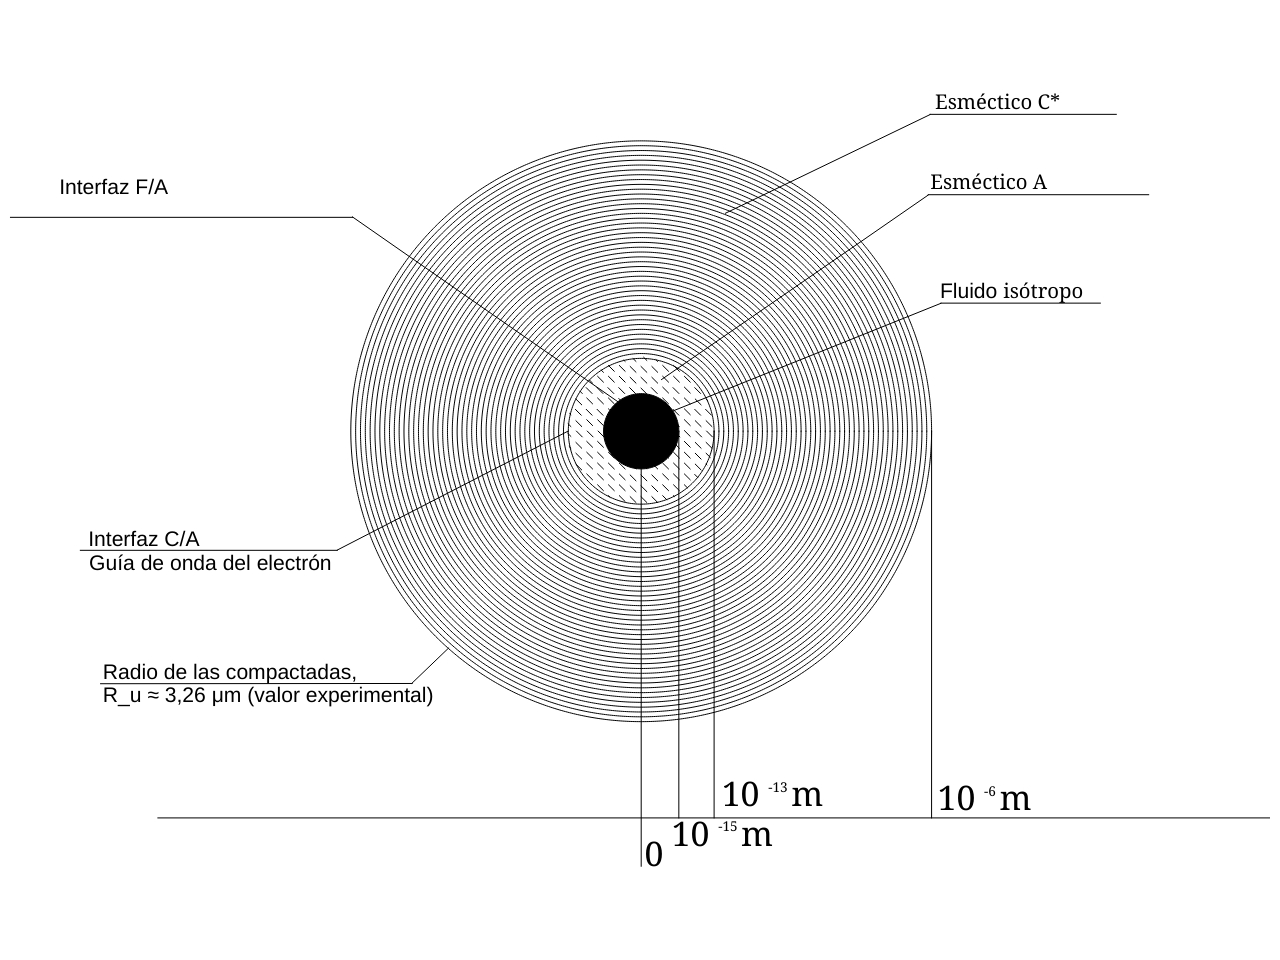
\includegraphics[width=\textwidth]{fig01_fases.jpg}
  \caption{}\label{fig:fases-a}
\end{subfigure}\hfill
\begin{subfigure}[b]{0.46\textwidth}
  \centering
  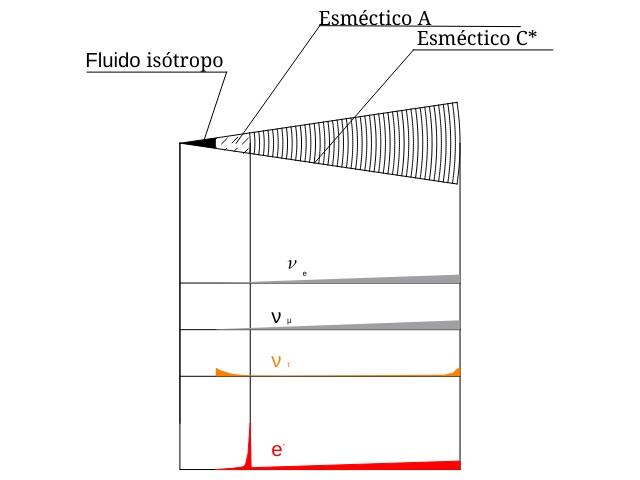
\includegraphics[width=\textwidth]{fig02_perfiles.jpg}
  \caption{}\label{fig:fases-b}
\end{subfigure}
\caption{Ilustración del postulado~4; esquema, no a escala. (a)~Las tres fases a lo largo de $\xi$ en el plano compacto, con las capas del esméctico~\Cst{} como circunferencias $\xi=\text{cte}$; el radio exterior es $R_u\approx 3,26~\mu\mathrm{m}$, valor experimental. La inclinación de las capas del \Cst{} y su precesión quiral no se ven en este corte. (b)~Dónde vive cada pulsación. Los neutrinos ligeros crecen hacia $R_u$, con la forma de las Bessel modificadas de orden~$\tfrac12$ con que se calculan sus masas. El electrón tiene su pico en la interfaz \Cst/A, a ${\sim}10^{-13}$~m, que coincide con $\xi_0=\hbar/(2mc)=1,93\times10^{-13}$~m (comprobación de coherencia interna); su cola no es su campo sino una envoltura de tipo neutrínico que se extiende por el \Cst{} hasta $R_u$ \st{H}.}
\label{fig:fases}
\end{figure}

\begin{figure}[!htb]
\centering
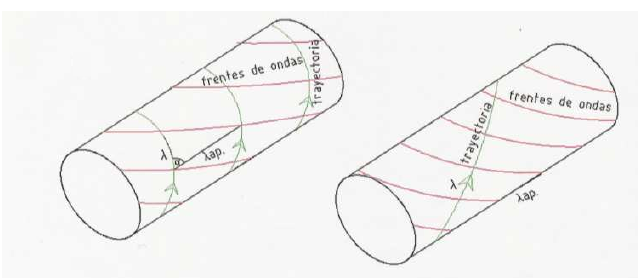
\includegraphics[width=0.85\textwidth]{fig03_cilindro.png}
\caption{Ilustración del postulado~6. La capa es un cilindro formado por la circunferencia compacta y una dirección extendida. La pulsación circula siempre sobre ella: en reposo la trayectoria es una circunferencia y los frentes de onda son paralelos al eje (longitud de onda aparente infinita); en movimiento la trayectoria es una hélice sobre la misma capa (izquierda, poco inclinada; derecha, más inclinada), y la longitud de onda aparente $\lambda_{\mathrm{ap}}$ a lo largo del eje se acorta al aumentar la inclinación, como la longitud de onda de de~Broglie. El cilindro es plano: al desenrollarlo la hélice es una recta, y el marco de la pulsación no gira al recorrerla.}
\label{fig:cilindro}
\end{figure}
% =====================================================================
\section{Consecuencias de los postulados}

\apartado{Separación de variables entre las soluciones en las compactadas y extendidas.}

\begin{itemize}[leftmargin=*]
\item \textbf{Caso lineal \st{D}.} Si la sección compacta es la misma en todos los puntos de las extendidas (postulado~1), la ecuación de ondas lineal separa exactamente en $H=\Phi(\xi,\eta)\,\Psi(\vb{x})\,e^{-i\omega t}$. La sección compacta da el perfil transversal (Bessel modificadas en $\xi$, $e^{i\eta/2}$ en $\eta$) y el corte $k_c$; las extendidas, $\nabla^2\Psi+(\omega^2/c^2-k_c^2)\Psi=0$, que es la ecuación de Klein--Gordon con masa $m=\hbar k_c/c$. Cada punto de las extendidas ve la sección compacta completa y perpendicular.

\item \textbf{Caso no lineal \st{H}.} Hay un solo campo, $H=\Phi\Psi$, y una no linealidad del hyle depende de la amplitud local $|H|^2$, que mezcla las dos partes: un término como $|H|^2H$ no separa exactamente. Que la física sea distinta en cada bloque (anisotropía extrema y permeación nula en $\xi,\eta$; hyle casi isótropo en las extendidas) cambia los coeficientes, pero no evita la mezcla. La separación se recupera de forma aproximada cuando la envolvente varía despacio frente a la sección compacta, como en una fibra óptica: el perfil transversal lo fija la guía lineal, y al promediar sobre la sección la envolvente obedece
\[
\nabla^2\Psi+\Bigl(\frac{\omega^2}{c^2}-k_c^2\Bigr)\Psi-g_{\mathrm{ef}}\,|\Psi|^2\Psi=0,
\qquad
g_{\mathrm{ef}}=g\,\frac{\int|\Phi|^4}{\int|\Phi|^2},
\]
el equivalente del «área efectiva» de las fibras (Agrawal, 2019). El error es del orden de $(\xi_0/L)^2$, con $L$ el tamaño de la envolvente: pequeño en un átomo ($L\approx a_0\approx 270\,\xi_0$), pero no a la escala de Compton, donde la aproximación deja de valer. En la práctica, las soluciones de las compactadas y de las extendidas se obtienen por separado, cada una con sus constantes. Queda abierto \st{A}: las nucleaciones, que dan el potencial de Mathieu, también dependen de la amplitud local, así que donde $\Psi$ es pequeña serían más débiles; hay que comprobar que eso no cambia el corte $k_c$, quizá porque el umbral las fija en cuanto se supera.

\item \textbf{Consecuencia física \st{D, dados los postulados 1 y 8}.} Como los campos de las interacciones (el arrastre en $\eta$ y el cambio de índice) no tienen modos propios en las compactadas (postulado~8), en las extendidas obedecen una ecuación en 3D y las leyes de fuerza no cambian por debajo de $R_u$; la parte compacta fijaría solo la intensidad de los acoplamientos ($\alpha$, $G$), que este trabajo no deriva. Los límites de dimensiones extra tipo ADD, que cuentan gravitones que se propagan por las compactadas, no se aplicarían directamente (sección~5, punto~9). La separación es necesaria para esto, pero no suficiente.
\end{itemize}

\apartado{Orden $\tfrac12$} (consecuencia de los postulados 1, 3, 4 y 6). La pulsación es antiperiódica a lo largo de $\eta$: media longitud de onda por vuelta \st{D}. Las capas son circunferencias concéntricas que llenan el plano compacto hasta su centro, el núcleo fluido (postulados 1 y~4), así que cada una rodea un disco; el marco de la pulsación está anclado a ellas, tangente a su circunferencia (postulado~6), y al dar una vuelta gira $360^\circ$ respecto a un marco fijo; y la pulsación es un espinor (postulado~3), que cambia de signo cuando su marco gira $360^\circ$. Por tanto el espinor es antiperiódico y el modo más bajo es el $\tfrac12$, no el entero: es la estructura de espín que hereda la frontera de un disco. Los modos enteros solo serían posibles si la circunferencia no rodeara nada, como en un toro sin centro. Precedente: en la «burbuja de la nada» de Witten (1982) la dimensión compacta se cierra sobre un punto, y eso solo es posible con fermiones antiperiódicos.

% ---------------------------------------------------------------------
\setcounter{subsection}{-1}
\subsection{Soluciones en las dimensiones compactadas}

En el plano compacto, $\eta$ es la dirección angular (a lo largo de las capas) y $\xi$ la radial (a través de ellas). La pulsación circula en $\eta$ con orden~$\tfrac12$ (deducido al principio de esta sección). En $\xi$ el sustrato no admite propagación (postulado~1), así que el perfil radial no oscila: no tiene nodos y crece, decrece o combina ambas cosas \st{H, consecuencia del postulado~1 y del orden~$\tfrac12$}. Sin nodos solo caben cuatro formas, y cada una se asocia a un tipo de pulsación según dónde se concentra respecto a las fases del postulado~4:

\begin{center}
\small
\begin{tabularx}{\textwidth}{@{}l Y Y Y Y@{}}
\toprule
Tipo & Forma del perfil en $\xi$ & Dónde vive & Pulsación & Estatus \\
\midrule
I & Creciente hacia el borde exterior (Bessel modificadas de orden~$\tfrac12$) & Dentro del esméctico~\Cst, hasta $R_u$ & $\nu_e$, $\nu_\mu$ & Masas calculadas con $R_u$ experimental \st{N} \\
\addlinespace
II & Decreciente hacia el borde exterior & Junto a la interfaz interior (fluido/A) & Soluciones hadrónicas (ondas de superficie) & Fuera de este trabajo; con las condiciones de contorno de los leptones no dan ninguna solución \st{N} \\
\addlinespace
IIbis & En U: mínimo interior, máximos en los dos extremos & Atraviesa todo el plano compacto & $\nu_\tau$ & Condición topológica (Floquet $\nu=\tfrac12$, $a=0$), sin depender de $\xi_0$ \st{D dentro de Mathieu} \\
\addlinespace
III & Creciente y luego decreciente, con cúspide & Interfaz A/\Cst & Electrón & Onda de interfaz, cúspide en $\xi_0=\hbar/(2mc)$ \st{H} \\
\bottomrule
\end{tabularx}
\end{center}

\textbf{Los neutrinos} son soluciones del propio esméctico~\Cst: no tienen una interfaz que los fije y se extienden hasta $R_u$, por eso su masa es tan pequeña y depende de $R_u$. \textbf{El electrón} es una onda de interfaz: la interfaz A/\Cst{} fija su radio $\xi_0$ y, con él, su masa y su carga. La mayor parte de su intensidad está del lado de~A, y por sí sola no tendría una posición radial definida: «caería» hacia el interior. Lo que la fija es su envoltura neutrínica, la cola evanescente que se adentra en \Cst: el perfil en A y la cola en \Cst{} tienen que empalmar en la interfaz, como una onda superficial ligada a la frontera entre dos medios, y esa condición de empalme es la que fija $\xi_0$ \st{H; el cálculo del empalme no está hecho en este trabajo}. Esto es lo que hace universal la carga (sección~5, punto~7). \textbf{El $\nu_\tau$} no está ligado a una escala sino a una condición topológica: une el interior con el exterior.

\apartado{Masas de los neutrinos.} Salen del orden de las centésimas de eV y dependen de $R_u$, que es un valor experimental y no está fijado de forma independiente \st{N, condicionado a $R_u$}. La comparación detallada con los datos de oscilaciones queda fuera de este trabajo \st{A}.

\apartado{Origen de la ecuación de Mathieu.} El paso de la ecuación de Bessel (círculo; es la de Mathieu con $q=0$, la de los neutrinos ligeros) a la de Mathieu con $q\neq0$, necesario para el electrón y el $\nu_\tau$, se atribuye a un potencial periódico que la propia pulsación genera en el sustrato, y no a una deformación elíptica real. El mecanismo es autoconsistente. En un potencial de periodo $\pi$ en $\eta$ (dos nucleaciones opuestas, $\cos2\eta$), la solución de Floquet tiene la forma $\Psi=e^{i\nu\eta}P(\eta)$, con $P$ de periodo $\pi$, así que su intensidad $|\Psi|^2=|P|^2$ tiene periodo $\pi$ para cualquier $\nu$, también para el orden~$\tfrac12$: una pulsación que circula en un solo sentido tiene dos máximos de intensidad por vuelta \st{D}. Si en esos máximos la intensidad supera un umbral del sustrato, amplificado cerca del punto tricrítico, aparecen dos nucleaciones opuestas, que generan justo el potencial $\cos2\eta$ que sostiene la solución: la pulsación crea el potencial que la mantiene \st{H, sin mecanismo cerrado}. La línea que une las dos nucleaciones es la que interviene en la lectura geométrica del espín. Precedente físico de una respuesta no lineal con umbral en la que una onda genera, a través de burbujas, una frecuencia distinta de la que la excita: la emisión subarmónica de las burbujas de cavitación (Prosperetti, 1975).

\apartado{Por qué el orden $\tfrac12$ puede circular} \st{D, teoría de Floquet y Bloch}. Una onda que circula en un solo sentido es la suma de dos ondas estacionarias en cuadratura, desplazadas un cuarto de longitud de onda y un cuarto de periodo: $\cos(k\eta)\cos(\omega t)+\operatorname{sen}(k\eta)\operatorname{sen}(\omega t)=\cos(k\eta-\omega t)$, como el campo giratorio de un motor de inducción con dos bobinados a $90^\circ$. Por eso el espinor es complejo: su parte real y su parte imaginaria son esas dos ondas. Con las dos nucleaciones, el potencial $\cos2\eta$ hace que la pulsación se comporte como una onda en un canal con obstáculos periódicos. Con orden entero la onda está en el borde de una banda (reflexión de Bragg): las dos ondas estacionarias, la que tiene los máximos sobre las nucleaciones y la que los tiene entre ellas, tienen frecuencias distintas, no pueden combinarse y nada circula. Con orden~$\tfrac12$ la onda está en el centro de la banda: las dos tienen la misma frecuencia y se combinan en una onda que circula en un solo sentido, y ese sentido es el signo de la carga. Con $|q|$ grande, entre las nucleaciones la onda es evanescente: su intensidad decae exponencialmente, pero no se anula, y esa cola mantiene unidas las dos nucleaciones, como la luz que atraviesa una capa fina de aire entre dos prismas (reflexión total frustrada). La circulación es de fase: la onda está en las dos nucleaciones a la vez y su fase avanza de una a otra. La intensidad no se anula en ningún punto, porque el caudal de la circulación, $j=|\Psi|^2\,d\varphi/d\eta$, es constante en toda la vuelta (es el wronskiano de la parte real y la imaginaria, que no pueden anularse a la vez), como en un canal: donde la intensidad es pequeña, la fase avanza deprisa. Un nodo sería una sección nula con caudal no nulo; por eso la circulación, es decir, la carga, y la ausencia de nodos son la misma cosa \st{D}. Las ondas estacionarias de orden entero, en cambio, sí tienen nodos, aunque solo puntuales. La anchura de la banda, que mide ese acoplamiento, decae como una exponencial de $\sqrt{|q|}$ ($2\times10^{-4}$ con $q=-10$; figura~\ref{fig:mathieu}).

\apartado{Ondas de un sentido y de dos sentidos.} Del párrafo anterior sale una distinción entre dos tipos de onda. Donde hay nucleaciones, el orden~$\tfrac12$ circula en un solo sentido: es la pulsación de espín~$\tfrac12$, con carga si está en la interfaz. Los órdenes enteros solo existen como ondas estacionarias, es decir, como superposición de los dos sentidos, y no tienen circulación neta \st{D, dentro del modelo}. Identificar esta distinción con la de fermiones y bosones es una hipótesis \st{H}. Dos pulsaciones de orden~$\tfrac12$ que circulan en sentidos opuestos se combinan en una onda de dos sentidos, que sería la versión ondulatoria de que dos fermiones formen un bosón (deuterón, helio-4). El campo (postulado~9) no es de dos sentidos en $\eta$: su circulación en $\eta$ tiene el sentido de la carga, porque si fuera de dos sentidos el campo eléctrico sería nulo. Lo que tiene dos sentidos es su forma en las extendidas, la onda estacionaria esférica, suma de una entrante y una saliente. La distinción entre uno y dos sentidos hay que hacerla, por tanto, dirección por dirección. Dos matices \st{A}: (i)~lo que da el espín~$\tfrac12$ es la antiperiodicidad, no el sentido único, porque una onda de orden~$\tfrac12$ en los dos sentidos seguiría cambiando de signo en una vuelta: el orden es la causa, y el sentido de circulación su consecuencia a través de la banda; (ii)~sin nucleaciones ($q\approx0$, neutrinos ligeros) no hay banda prohibida y los órdenes enteros también podrían circular (sección~5, punto~9), y un bosón cargado necesitaría amplitudes distintas en cada sentido, es decir, una circulación neta que ya no es estacionaria pura. El desarrollo para partículas compuestas queda para el trabajo sobre hadrones.

\begin{figure}[!htb]
\centering
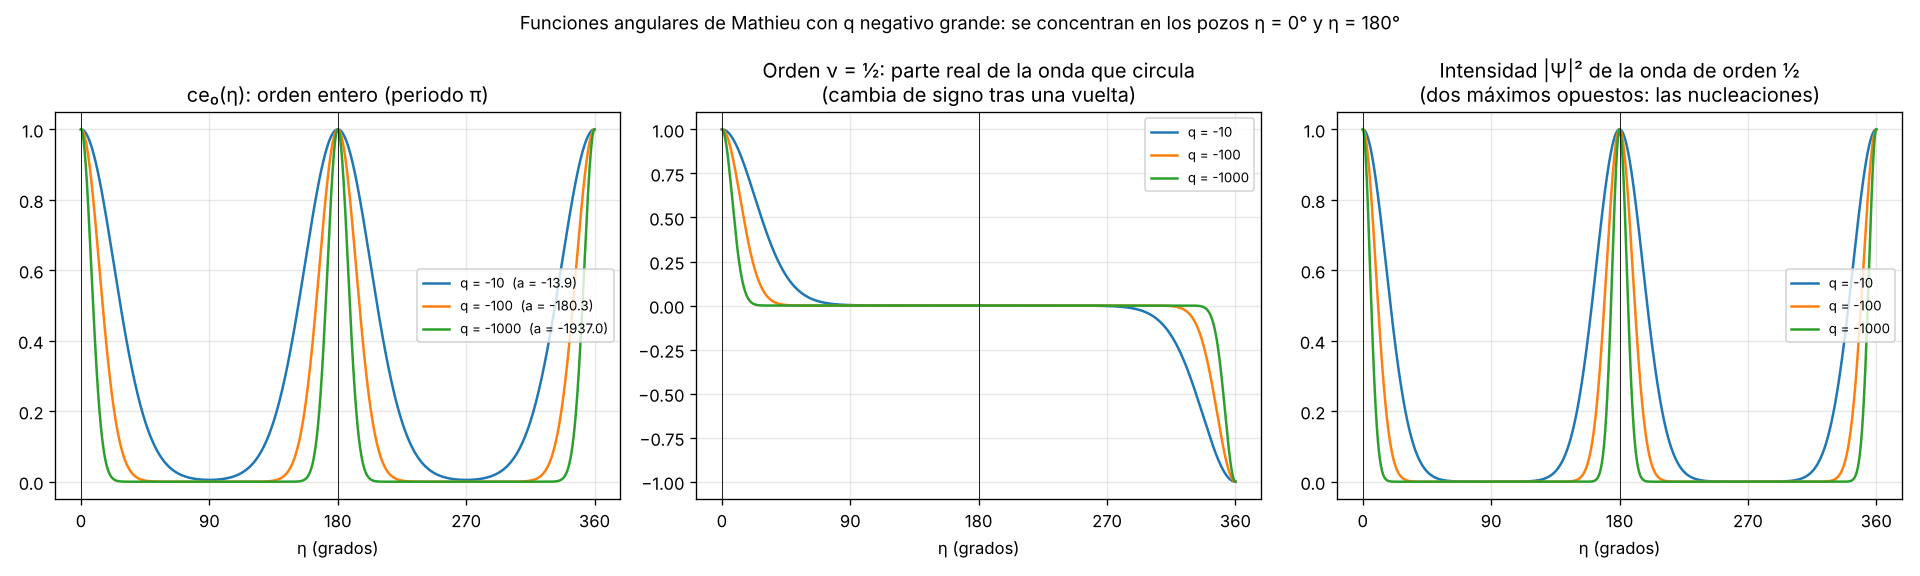
\includegraphics[width=\textwidth]{fig04_mathieu.png}
\caption{Funciones angulares de Mathieu para $q=-10$, $-100$ y $-1000$. Con $q$ negativo los pozos del potencial están en $\eta=0^\circ$ y $180^\circ$, y la función se concentra en ellos tanto más cuanto mayor es $|q|$. Izquierda: orden entero ($\mathrm{ce}_0$). Centro: parte real de la onda de orden~$\tfrac12$ que circula en un solo sentido; vale $+1$ en $0^\circ$ y $-1$ en $360^\circ$ (cambio de signo tras una vuelta), y en $180^\circ$ es imaginaria pura (fase de un cuarto de ciclo). Derecha: intensidad $|\Psi|^2$ de esa onda, con dos máximos iguales y opuestos, que son las dos nucleaciones. Con $|q|$ grande los valores característicos de los órdenes $0$ y $\tfrac12$ coinciden (la diferencia es de $2\times10^{-4}$ con $q=-10$ y despreciable con $q=-100$): el orden~$\tfrac12$ no lo selecciona la energía, sino la antiperiodicidad (sección~2). Elaborada con \prog{mathieu\_q.py} (método de Hill).}
\label{fig:mathieu}
\end{figure}

\begin{figure}[!htb]
\centering
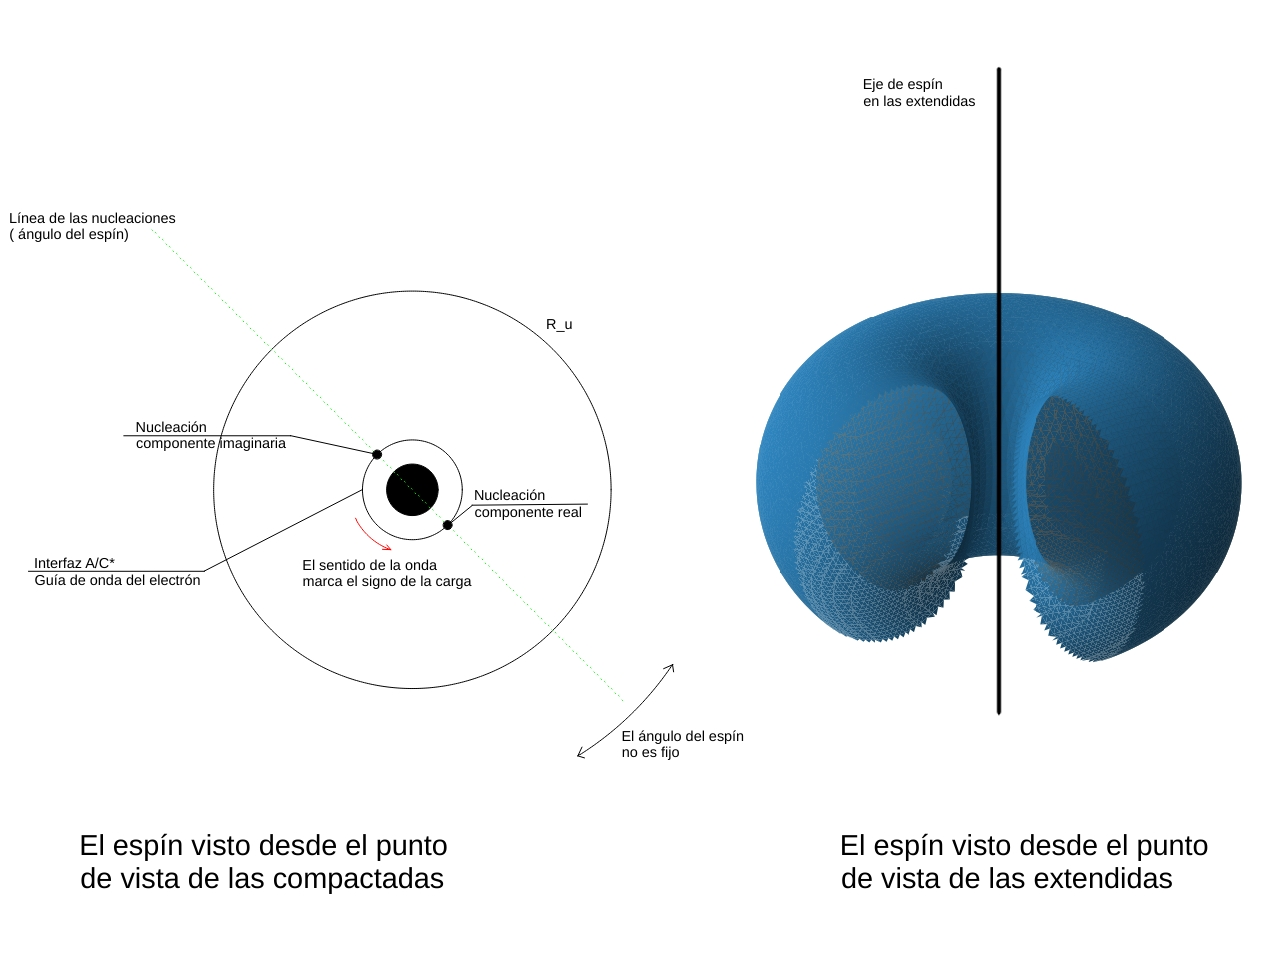
\includegraphics[width=0.75\textwidth]{fig05_espin_dos_lados.jpg}
\caption{El espín visto desde los dos lados. Izquierda, el plano compacto: el núcleo fluido (negro), la interfaz A/\Cst{} donde circula el electrón y el borde $R_u$. La onda circula en un solo sentido, que marca el signo de la carga, y forma dos nucleaciones opuestas; la línea que las une da el ángulo del espín, que no es fijo. En un instante dado, la onda está desfasada un cuarto de ciclo entre las dos nucleaciones (componente real en una, imaginaria en la otra), como muestra el panel central de la figura~\ref{fig:mathieu}. Derecha, las extendidas: el hopfión con su eje, que es el eje del espín. Juntos forman la fibración de Hopf: un eje en las extendidas y un ángulo en las compactadas.}
\label{fig:espin-dos-lados}
\end{figure}

Con los postulados 2, 3, 5 y 6 y el orden~$\tfrac12$, la reducción a $3+1$ dimensiones da la ecuación de Dirac con $g=2$; sin el anclaje del postulado~6 (Kaluza--Klein ordinario) daría $g=1$. Todo lo de esta sección es \st{D} dados los postulados.

\apartado{Deducción paso a paso.} Cada paso indica de qué postulado sale y con qué estatus. Se usa $c=1$ en las ecuaciones intermedias y $\hbar$, $c$ explícitos en los resultados; $\eta$ es la longitud de arco a lo largo de la capa, de modo que una vuelta mide $2\pi\xi_0$.

\textbf{Paso 1. La ecuación en $4+1$ dimensiones} \st{postulado~3}. La pulsación es un espinor $\Psi$ que obedece una ecuación de ondas de primer orden y sin masa en $(t,x,y,z,\eta)$:
\begin{equation}
\gamma^0\frac{\partial\Psi}{\partial t}+\gamma^x\frac{\partial\Psi}{\partial x}+\gamma^y\frac{\partial\Psi}{\partial y}+\gamma^z\frac{\partial\Psi}{\partial z}+\gamma^\eta\frac{\partial\Psi}{\partial\eta}=0 .
\label{eq:paso1}
\end{equation}
Los coeficientes son cinco matrices de $4\times4$ que se anticonmutan dos a dos: $\gamma^A\gamma^B+\gamma^B\gamma^A=2g^{AB}$, con $g=\operatorname{diag}(1,-1,-1,-1,-1)$. En $4+1$ dimensiones bastan matrices de $4\times4$, porque la quinta es el producto de las otras cuatro: $\gamma^\eta\propto\gamma^0\gamma^x\gamma^y\gamma^z$. Al aplicar la ecuación dos veces, los productos cruzados se cancelan por la anticonmutación y queda, para cada componente de $\Psi$:
\begin{equation}
\frac{\partial^2\Psi}{\partial t^2}-\nabla^2\Psi-\frac{\partial^2\Psi}{\partial\eta^2}=0 .
\label{eq:ondas5}
\end{equation}
La ecuación de primer orden es la «raíz cuadrada» de la de ondas: la pulsación avanza a $c$ y no tiene masa en el hyle (postulado~2). Es el procedimiento de Dirac (1928), que buscó una ecuación de primer orden cuyo cuadrado fuera la de Klein--Gordon. Aquí la ecuación de primer orden hace el papel de la de Dirac, pero su cuadrado es la ecuación de ondas sin masa en $4+1$ dimensiones; Klein--Gordon, con su masa, aparece al reducir a $3+1$ (Paso~3) \st{D}.

\textbf{Paso 2. La condición en $\eta$} \st{D, orden~$\tfrac12$, principio de esta sección}. La pulsación es antiperiódica a lo largo de la capa, $\Psi(\eta+2\pi\xi_0)=-\Psi(\eta)$, así que se puede escribir $\Psi=e^{ik\eta}\chi(t,x,y,z)$, con
\begin{equation}
k=\pm\frac{n+\tfrac12}{\xi_0},\quad n=0,\ 1,\ 2,\ \dots;
\qquad\text{modo más bajo: } k=\pm\frac{1}{2\xi_0} .
\label{eq:paso2}
\end{equation}
El signo de $k$ es el sentido de circulación en $\eta$. El perfil en la dirección radial $\xi$ (Bessel modificadas, apartado~2.0) fija en qué capa está la pulsación, pero no cambia lo que sigue.

\textbf{Paso 3. Aparece la masa} \st{D}. Al sustituir $\partial/\partial\eta$ por $ik$, el término en $\eta$ pierde la derivada:
\begin{equation}
\gamma^0\frac{\partial\chi}{\partial t}+\vb{\gamma}\cdot\nabla\chi+ik\,\gamma^\eta\chi=0 .
\label{eq:paso3}
\end{equation}
Aplicada dos veces da $(\partial_t^2-\nabla^2+k^2)\chi=0$: la relación de dispersión de una partícula con masa, $\omega^2=c^2p^2/\hbar^2+c^2k^2$. La frecuencia mínima, $c|k|$, es la frecuencia de corte de la guía de ondas del postulado~2, y la masa es
\begin{equation}
m=\frac{\hbar|k|}{c}=\frac{\hbar}{2\xi_0c}
\qquad\Longleftrightarrow\qquad
\xi_0=\frac{\hbar}{2mc} .
\label{eq:masa}
\end{equation}
El término de masa aparece multiplicado por $\gamma^\eta$ y no por la unidad, como en la forma habitual de Dirac. Como $\gamma^\eta$ es proporcional al producto de las otras cuatro, un cambio de fase constante entre las componentes de $\chi$ lo lleva a la forma habitual sin cambiar ningún observable \st{D, estándar en Kaluza--Klein}. La relación $\xi_0=\hbar/(2mc)$ vale tal cual para el electrón, que es una onda de interfaz pura, y fija con su masa el radio de la interfaz A/\Cst: $\xi_{\mathrm{interfaz}}\approx1,93\times10^{-13}$~m. En otras partículas no se puede invertir así, porque su masa incluye otras contribuciones (la vibración de las nucleaciones en el muón y el tauón, sus demás partes en las epícimas).

\textbf{Paso 4. La carga y el campo} \st{D, dado el postulado~5}. El arrastre del hyle a lo largo de $\eta$ desplaza localmente el origen de $\eta$. En la ecuación entra como
\begin{equation}
\partial_\mu\;\longrightarrow\;\partial_\mu-\kappa A_\mu\,\partial_\eta ,
\label{eq:arrastre}
\end{equation}
donde $A_\mu$ describe el arrastre y $\kappa$ es una constante de acoplamiento. Sobre $e^{ik\eta}$ esto da $\partial_\mu-i\kappa kA_\mu$: el acoplamiento mínimo de una carga $q\propto k$ a un potencial $A_\mu$. El signo de la carga es el sentido de circulación. El $k$ que da la carga es el de la onda que circula en la interfaz A/\Cst, $k=1/(2\xi_{\mathrm{interfaz}})$, el mismo para toda partícula que tenga una parte en la interfaz: el electrón entero, las epícimas pesadas en parte. Por eso la carga es universal, y las partículas sin esa parte, como los neutrinos dentro de \Cst, no la tienen (postulado~5) \st{H, coherente con el postulado~5}. Cada interacción es universal dentro de su capa: la eléctrica en la interfaz A/\Cst, la fuerte en la superficie del núcleo fluido. Desplazar el origen de $\eta$ de forma distinta en cada punto equivale a una transformación gauge,
\begin{equation}
\eta\;\longrightarrow\;\eta+\lambda(x)
\qquad\Longleftrightarrow\qquad
A\;\longrightarrow\;A-\nabla\lambda/\kappa ,
\label{eq:gauge}
\end{equation}
de modo que la invariancia gauge del electromagnetismo es la libertad de elegir el origen de $\eta$ en cada punto \st{D}.

\textbf{Paso 5. Espín $\tfrac12$ y $g=2$} \st{D, dados los postulados 3 y~6}. Con $D_\mu=\partial_\mu-iqA_\mu$, aplicar la ecuación dos veces ya no da solo la ecuación de ondas: como las $D_\mu$ no conmutan entre sí cuando hay campo, aparece un término adicional proporcional a $F_{\mu\nu}$ y a los productos $\gamma^\mu\gamma^\nu$. En el límite de velocidades pequeñas es la energía de un momento magnético en el campo $\vb{B}$ con $g=2$ exacto (Dirac, 1928). Y como $\Psi$ es un espinor, el espín es~$\tfrac12$.

\apartado{El papel del postulado 6} \st{D, resultados conocidos}. En Kaluza--Klein ordinario el campo es una deformación de la geometría, el marco local gira con ella y la conexión de espín añade a la ecuación un término $(\kappa/8)F_{\mu\nu}\gamma^\mu\gamma^\nu\gamma^\eta\Psi$ que cambia el momento magnético: todos los estados masivos en $3+1$ dimensiones, es decir, los que circulan en la dimensión compacta como nuestra pulsación, tienen $g=1$ (Hosoya et al., 1984; Duff, Liu y Rahmfeld, 1998). Que la pulsación no tenga masa en el hyle no la libra de este resultado: es precisamente el caso que describe. Con el marco anclado a las capas, el arrastre es flujo sobre las capas y no deformación, el transporte no gira el marco (conexión de Weitzenböck), el término no aparece y queda el acoplamiento mínimo puro: $g=2$. Es el único ingrediente no estándar de la deducción.

\apartado{Lo que ya da Kaluza--Klein y lo que añade el sustrato.} En Kaluza--Klein ordinario la carga es ya la circulación en la dimensión compacta, y su cuantización sale de que la circunferencia se cierre (Klein, 1926): para que exista la carga y esté cuantizada no hace falta sustrato \st{D}. Lo que añade el sustrato es, por un lado, $g=2$ (postulado~6); por otro, separar la carga de la masa. Con un único radio, como en Kaluza--Klein ordinario, carga y masa son las dos proporcionales a $k$: todas las partículas cargadas tendrían el mismo cociente carga/masa, y para la carga del electrón la masa tendría que ser del orden de la de Planck, uno de los problemas que hicieron abandonar Kaluza--Klein como teoría del electrón. En el modelo, la carga sale solo de la onda de interfaz, con $k$ fijo, y la masa es la de la partícula entera, que puede tener otras partes y otras capas \st{H}.

La lista siguiente resume estos resultados y añade la lectura geométrica del espín.

\begin{enumerate}[label=\arabic*.,leftmargin=*]
\item \textbf{La ecuación.} $\gamma^0\partial_t\Psi+\vb{\gamma}\cdot\nabla\Psi+\gamma^\eta\partial_\eta\Psi=0$, con cinco matrices que se anticonmutan ($4\times4$; $\gamma^\eta=i\gamma^0\gamma^x\gamma^y\gamma^z$). Aplicada dos veces da la ecuación de ondas sin masa en $4+1$.

\item \textbf{Masa.} Con antiperiodicidad en $\eta$, $\Psi\propto e^{ik\eta}$, $k=\pm(n+\tfrac12)/\xi_0$. El modo más bajo da la ecuación de Dirac con masa $m=\hbar/(2\xi_0c)$, es decir $\xi_0=\hbar/(2mc)$. Perfil en la dirección radial $\xi$ \st{H, consecuencia del postulado~1}: el sustrato no admite propagación a través de las capas, así que el perfil en $\xi$ no oscila ni tiene nodos; su número de onda es imaginario ($k_\xi^2<0$) y las soluciones son las Bessel modificadas. Es una respuesta reactiva, evanescente, sin pérdidas: una amortiguación viscosa disipativa daría un número de onda complejo y la pulsación se apagaría. La masa es la frecuencia del modo completo, incluido ese perfil, y no $c\,k_\eta$: como no existe una pulsación sin perfil radial con la que comparar, la diferencia no es una energía de enlace, y el criterio de autoenlace nulo (que se refiere a la envolvente en las extendidas) no se ve afectado. Este signo se eligió por primera vez en un trabajo previo del autor (E.~López, «Matter as gravitational waves», preprint no publicado, ResearchGate), con el argumento de que las ondas en $\xi$ «saldrían del Universo»; el postulado~1 le da ahora un fundamento físico.

\item \textbf{Carga.} El signo de $k$ es el signo de la carga: las dos ondas de orden~$\tfrac12$ ($+\tfrac12$ y $-\tfrac12$) son partícula y antipartícula, con la misma $|k|$ y la misma masa.

\item \textbf{Invariancia gauge.} El arrastre entra como $\partial_\mu\to\partial_\mu-\kappa A_\mu\partial_\eta$; desplazar el origen de $\eta$ en cada punto ($\eta\to\eta+\lambda(x)$) equivale a $A\to A-\nabla\lambda/\kappa$.

\item \textbf{Espín $\tfrac12$.} $\Psi$ es un espinor de cuatro componentes: dos sentidos de circulación (carga) por dos orientaciones (espín). Lectura geométrica \st{H}: el espín es una dirección en las extendidas más el ángulo que forma, en el plano compacto, la línea que une las nucleaciones periódicas (fibración de Hopf). Si todo el conjunto, nucleaciones y onda, gira media vuelta o una vuelta entera ($\Delta\eta=\pi,2\pi$), que son los giros en los que el patrón de nucleaciones vuelve a coincidir consigo mismo, la onda $\Psi=e^{i\eta/2}P(\eta)$ queda multiplicada por $e^{-i\Delta\eta/2}$ \st{D}: tras media vuelta la línea se ve igual, pero la onda ha cambiado su fase un cuarto de ciclo ($-i$); tras una vuelta completa la geometría vuelve a ser la misma y la onda ha cambiado de signo ($-1$); hacen falta dos vueltas para volver al estado inicial. La simetría de la línea a media vuelta es una simetría del potencial, no un giro físico. Acoplamiento de los dos giros \st{H}: en la reformulación de la ecuación de Dirac con álgebra geométrica, la unidad imaginaria del espinor es el plano de giro del espín, y la fase es un ángulo de giro en ese plano con la ley de mitad de ángulo (Hestenes, 1990). Si la fase de la pulsación es su posición a lo largo de $\eta$, avanzar en $\eta$ es girar el marco en el plano del espín: una vuelta en el plano compacto corresponde a una vuelta completa del marco en las extendidas, con el cambio de signo. Los dos giros son una sola rotación doble, igual en dos planos perpendiculares. Identificar la fase de la carga con el giro del espín es una hipótesis del modelo; queda por comprobar que es compatible con que electrón y positrón tengan el mismo espín y carga opuesta \st{A}.

\item \textbf{$g=2$ con el sustrato, $g=1$ sin él (resultado central).}
  \begin{itemize}
  \item Kaluza--Klein ordinario: el marco $d\eta+\kappa A\cdot dx$ no cierra cuando $F\neq0$, y la conexión de espín añade $(\kappa/8)F_{\mu\nu}\gamma^\mu\gamma^\nu\gamma^\eta\Psi$; todos los estados masivos tienen $g=1$ (Duff, Liu y Rahmfeld, hep-th/9801072; término explícito en hep-ph/0203037).
  \item Con el marco anclado a las capas (postulado~6) el término no aparece (conexión de Weitzenböck): acoplamiento mínimo puro y $g=2$ exacto.
  \end{itemize}

\item \textbf{Dos electrones por orbital \st{H}.} En el espacio de espinores solo caben dos estados perfectamente distinguibles. Imagen geométrica: para espín opuesto, las líneas que unen las nucleaciones son perpendiculares, la máxima separación posible entre dos líneas en un plano, y coincide con la regla de la mitad del ángulo (estados opuestos, a $180^\circ$ en el espacio, son perpendiculares como espinores). Con esas líneas las ondas de orden~$\tfrac12$ casi no se solapan: el solapamiento es $0,05$ con $q=-10$, $1,6\times10^{-5}$ con $q=-100$ y del orden de $10^{-16}$ con $q=-1000$ \st{N}. Por eso dos electrones de espín opuesto pueden compartir orbital. Para espín paralelo, con la misma línea, la separación la da el desfase temporal: medio periodo es un factor $-1$, las dos ondas se anulan donde coincidirían y no se solapan; es la antisimetría de Pauli vista mecánicamente. Matiz: con $|q|$ muy grande incluso líneas a $45^\circ$ casi no se solapan, así que el «dos» sigue viniendo de las dos orientaciones del espinor, no solo del solapamiento. Condición abierta \st{A}: si el ángulo inicial entre líneas y el desfase deciden cómo se colocan dos electrones que se encuentran, el modelo tiene que reproducir las proporciones cuánticas; por ejemplo, la probabilidad de acabar con espín total~0 para dos espines cuyos ejes forman un ángulo $\theta$ es $(1-\cos\theta)/4$.
\end{enumerate}

\begin{figure}[!htb]
\centering
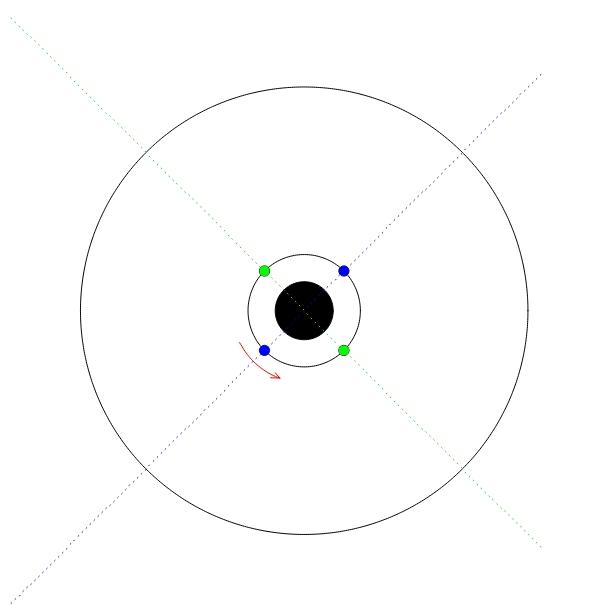
\includegraphics[width=0.48\textwidth]{fig06_dos_electrones.jpg}
\caption{Hipótesis: dos electrones de espín $+\tfrac12$ y $-\tfrac12$ compartiendo un orbital. Sus líneas de nucleación (verde y azul) son perpendiculares, la máxima separación posible entre dos líneas, y las dos ondas circulan en el mismo sentido (misma carga). Con esa disposición las ondas casi no se solapan (véase el punto «Dos electrones por orbital»).}
\label{fig:dos-electrones}
\end{figure}
% =====================================================================
\section{Estructura del leptón en las extendidas}

Se ha minimizado numéricamente la energía del director y se ha comprobado que forma un hopfión estable, con la energía de la literatura a menos del 1~\% (Sutcliffe, 2007), cuyo flujo es un anillo de vórtice con remolino; el giro en $\eta$ le añade la masa de Kaluza--Klein esperada y una cola de Yukawa dipolar. Todo \st{N}, con programas reproducibles (\prog{hopfion.cpp}, \prog{flujo.py}, \prog{hopfion\_eta.cpp}, \prog{cola\_angular.py}).

Para validar los cálculos numéricos realizados se ha utilizado una malla $150^3$ en una caja de 12 unidades de longitud y se ha estimado la energía de Faddeev--Skyrme $\int\bigl[\partial_i\vb{n}\cdot\partial_i\vb{n}+\tfrac12F_{ij}F_{ij}\bigr]$: $E/(32\sqrt2\,\pi^2)=1,219$ frente a ${\sim}1,21$ de la literatura (Sutcliffe, 2007), con una carga de Hopf $Q=-0,979$ y un virial $E_2/E_4=0,965$ \st{N}.

\apartado{Flujo.} Con la relación de Mermin--Ho (vorticidad = retorcimiento del director), el flujo del hopfión es un anillo de vórtice con remolino: 66~\% de la energía en la circulación poloidal y 34~\% en la toroidal, con momento angular neto alrededor del eje libre. Su helicidad es $16\pi^2Q$ \st{N}. El reparto no es una proporción fija: en el mapa de Hopf analítico tiende a 50~\% / 50~\%, y en el hopfión pasa del 66~\% de poloidal con $k=0$ al 67~\% con $k=0,5$ y al 68~\% con $k=1$ (\prog{reparto\_flujo.py}); depende de la forma del mínimo de energía, no de la topología \st{N}.

\apartado{Precedente: los átomos-vórtice de Kelvin.} Kelvin (1867) propuso que los átomos eran vórtices anudados en un fluido: el más simple, un anillo sin nudo; los demás, nudos cada vez más complicados, que Tait clasificó en las primeras tablas de nudos. El hopfión con $Q=1$ corresponde al anillo simple, pero con remolino: su núcleo no está anudado, mientras que cada línea de vorticidad es una curva $(1,1)$ sobre su toro y cualquier par de ellas está enlazado una vez. En el mismo modelo de Faddeev--Skyrme aparecen nudos de verdad a carga mayor: con $Q=7$ el mínimo de energía es un nudo de trébol (Battye y Sutcliffe, 1998; Faddeev y Niemi, 1997, que citan expresamente a Kelvin). A Kelvin le faltó la estabilidad: en un fluido ideal nada impide que un anillo se expanda o se deforme. Aquí la dan la topología y el término de cuarto orden.

\apartado{Precedentes del espín topológico.} Que un nudo de campos sin espín tenga espín~$\tfrac12$ no es una idea nueva. Finkelstein y Rubinstein (1968) mostraron que un solitón topológico puede tener espín semientero; Witten (1983) lo aplicó a los skyrmiones como modelo de bariones; y Krusch y Speight (2006) estudiaron si los hopfiones de Faddeev--Skyrme admiten espín semientero. La imagen de este trabajo, un eje en las extendidas (el del nudo) más un ángulo en la dimensión compacta (la línea de las nucleaciones), se apoya en esa línea y se sostendría aun sin el sustrato \st{H}. Lo que añade el sustrato es lo demás: $g=2$ (postulado~6), la separación entre carga y masa y la universalidad de la carga en la interfaz (sección~2), y las propias nucleaciones, que necesitan un umbral del medio.

\apartado{Un precedente en un sustrato real.} Volovik y Mineev (1977) estudiaron solitones con forma de partícula en las fases superfluidas del helio-3: sin singularidades, de tamaño y energía finitos y con un invariante topológico entero, entre ellos los de Hopf. Coinciden con este trabajo en varios puntos: obtienen el flujo de la textura con la relación de Mermin--Ho, escriben el invariante como la helicidad del flujo, $\int\vb{v}\cdot\operatorname{rot}\vb{v}$, y encuentran un campo de velocidades lejano dipolar, como el de un sólido que se mueve en un fluido ideal. Es decir, en un medio real hay nudos de la textura que se comportan como partículas, con flujo de Mermin--Ho y cola dipolar. Además, en la fase~A el solitón se estabiliza por su momento: al conservarlo deja de poder encogerse y su tamaño queda fijado sin términos de cuarto orden en el gradiente (sección~5, punto~13).

\begin{figure}[!htb]
\centering
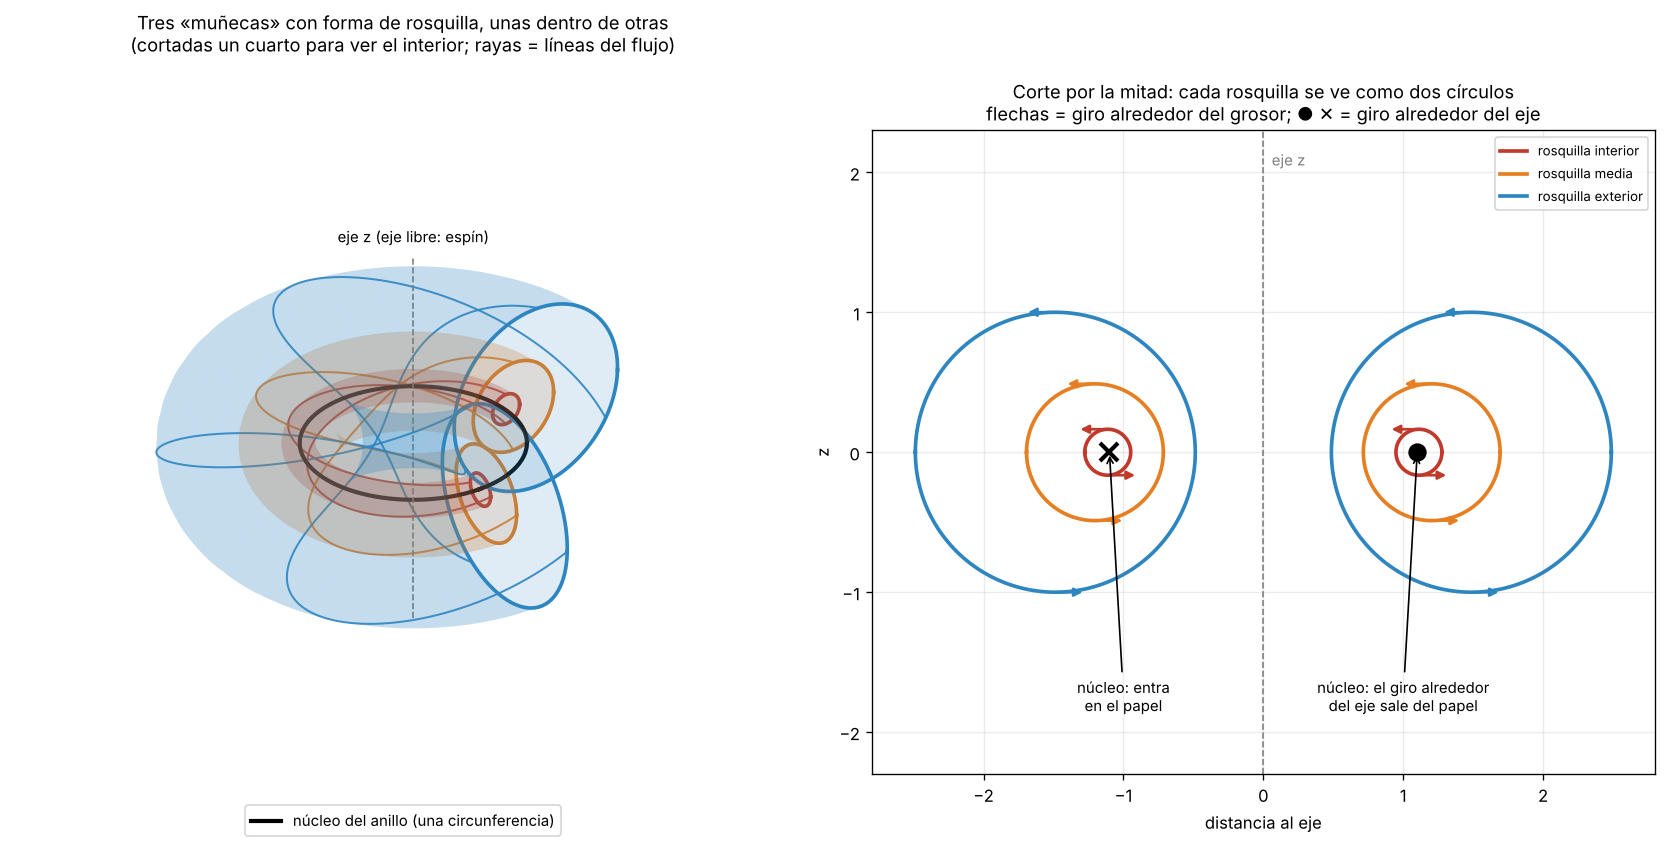
\includegraphics[width=0.9\textwidth]{fig07_toros.png}
\caption{Geometría del hopfión: las superficies de igual inclinación del director son toros anidados alrededor del núcleo del anillo (circunferencia negra), no concéntricos. Las líneas del flujo se enrollan a la vez alrededor del grosor (poloidal) y alrededor del eje $z$ (toroidal); su enlace es la carga de Hopf. Esquema cualitativo en coordenadas toroidales, no la solución numérica.}
\label{fig:toros}
\end{figure}

\begin{figure}[!htb]
\centering
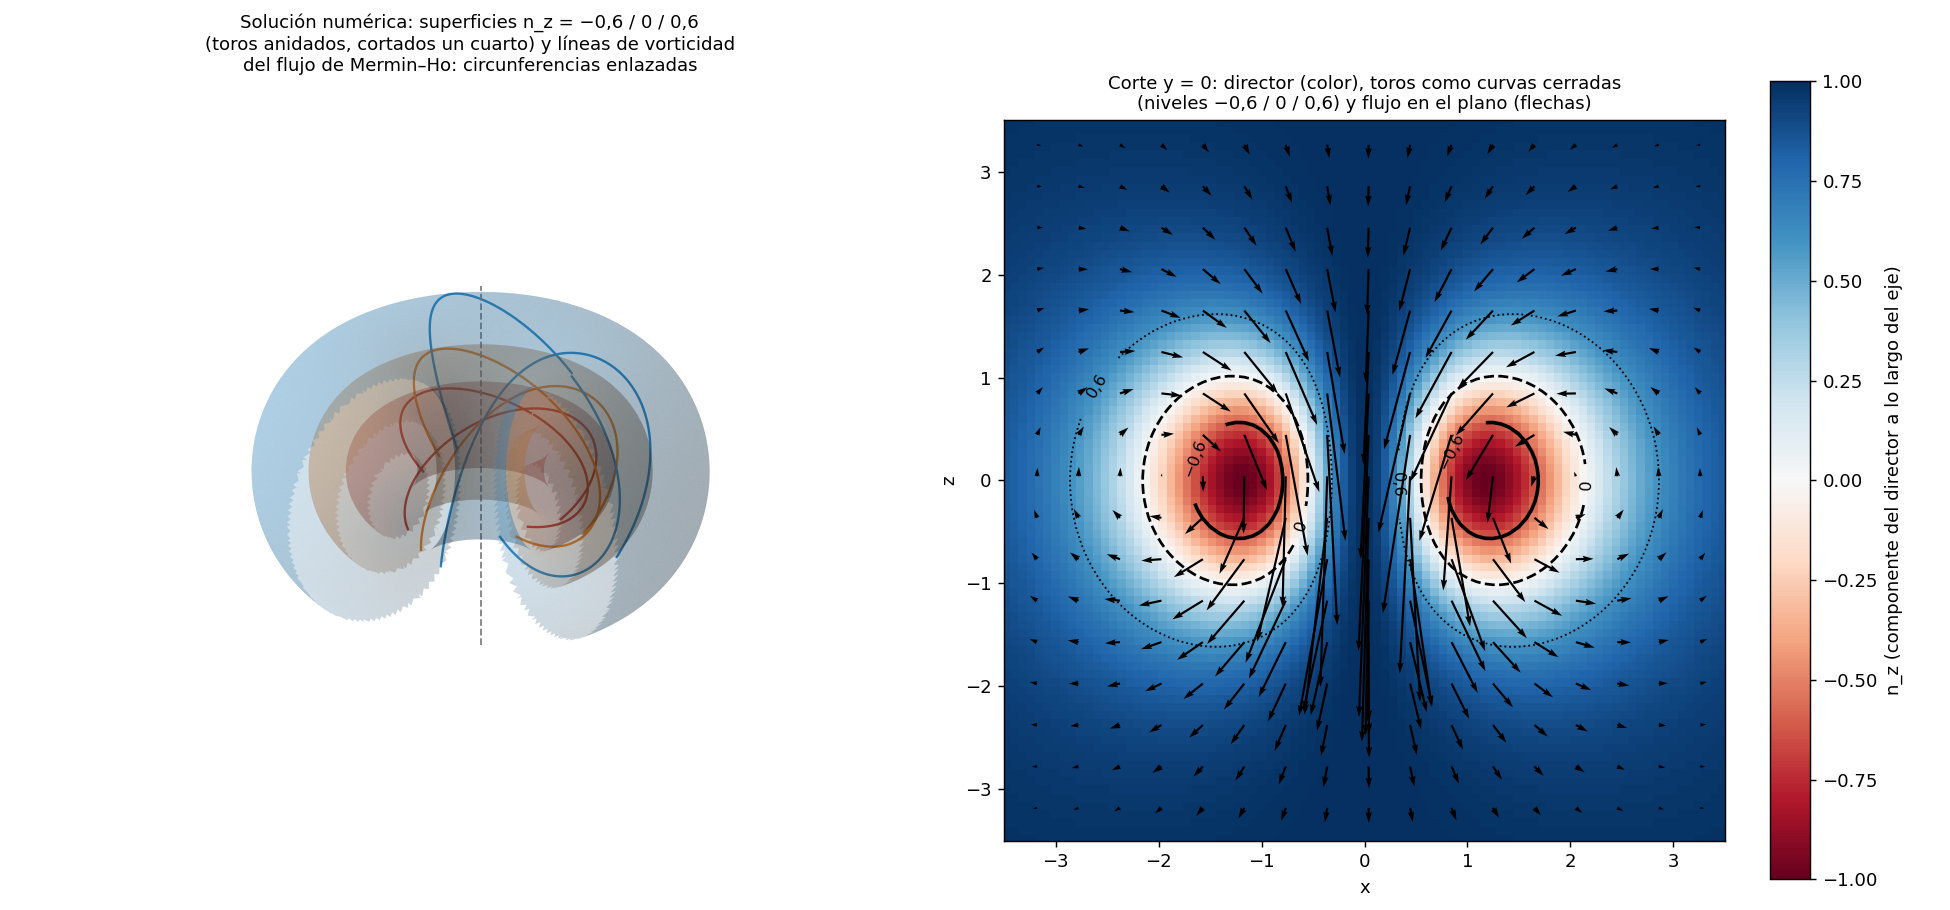
\includegraphics[width=\textwidth]{fig08_hopfion_k0.png}
\caption{Solución numérica del hopfión (malla $150^3$, caja de lado~12; la de $100^3$ da la misma figura). Izquierda: superficies $n_z=-0,6$, $0$ y $0,6$, toros anidados, cortados un cuarto; líneas de vorticidad del flujo de Mermin--Ho, que son circunferencias cerradas sobre cada toro y se enlazan entre sí (su enlace es la carga de Hopf). Derecha: corte por el plano $y=0$; en color, la componente del director a lo largo del eje ($-1$ en el núcleo del anillo, $+1$ en el reposo); en negro, las mismas superficies como curvas cerradas; flechas, el flujo en el plano, con el chorro por el centro. Unidades: todas las longitudes de esta sección ($r$, radios, caja) están en unidades de $\ell=\sqrt{\kappa_4/\kappa_2}$, el cociente entre la rigidez de cuarto orden y la rigidez del director; $k$ está en unidades de $1/\ell$ y las energías en unidades de $\sqrt{\kappa_2\kappa_4}$. El valor de $\ell$ en metros no está fijado (véase «Lo abierto», punto~5). Elaborada con \prog{figura\_hopfion.py}.}
\label{fig:hopf-k0}
\end{figure}

\begin{figure}[!htb]
\centering
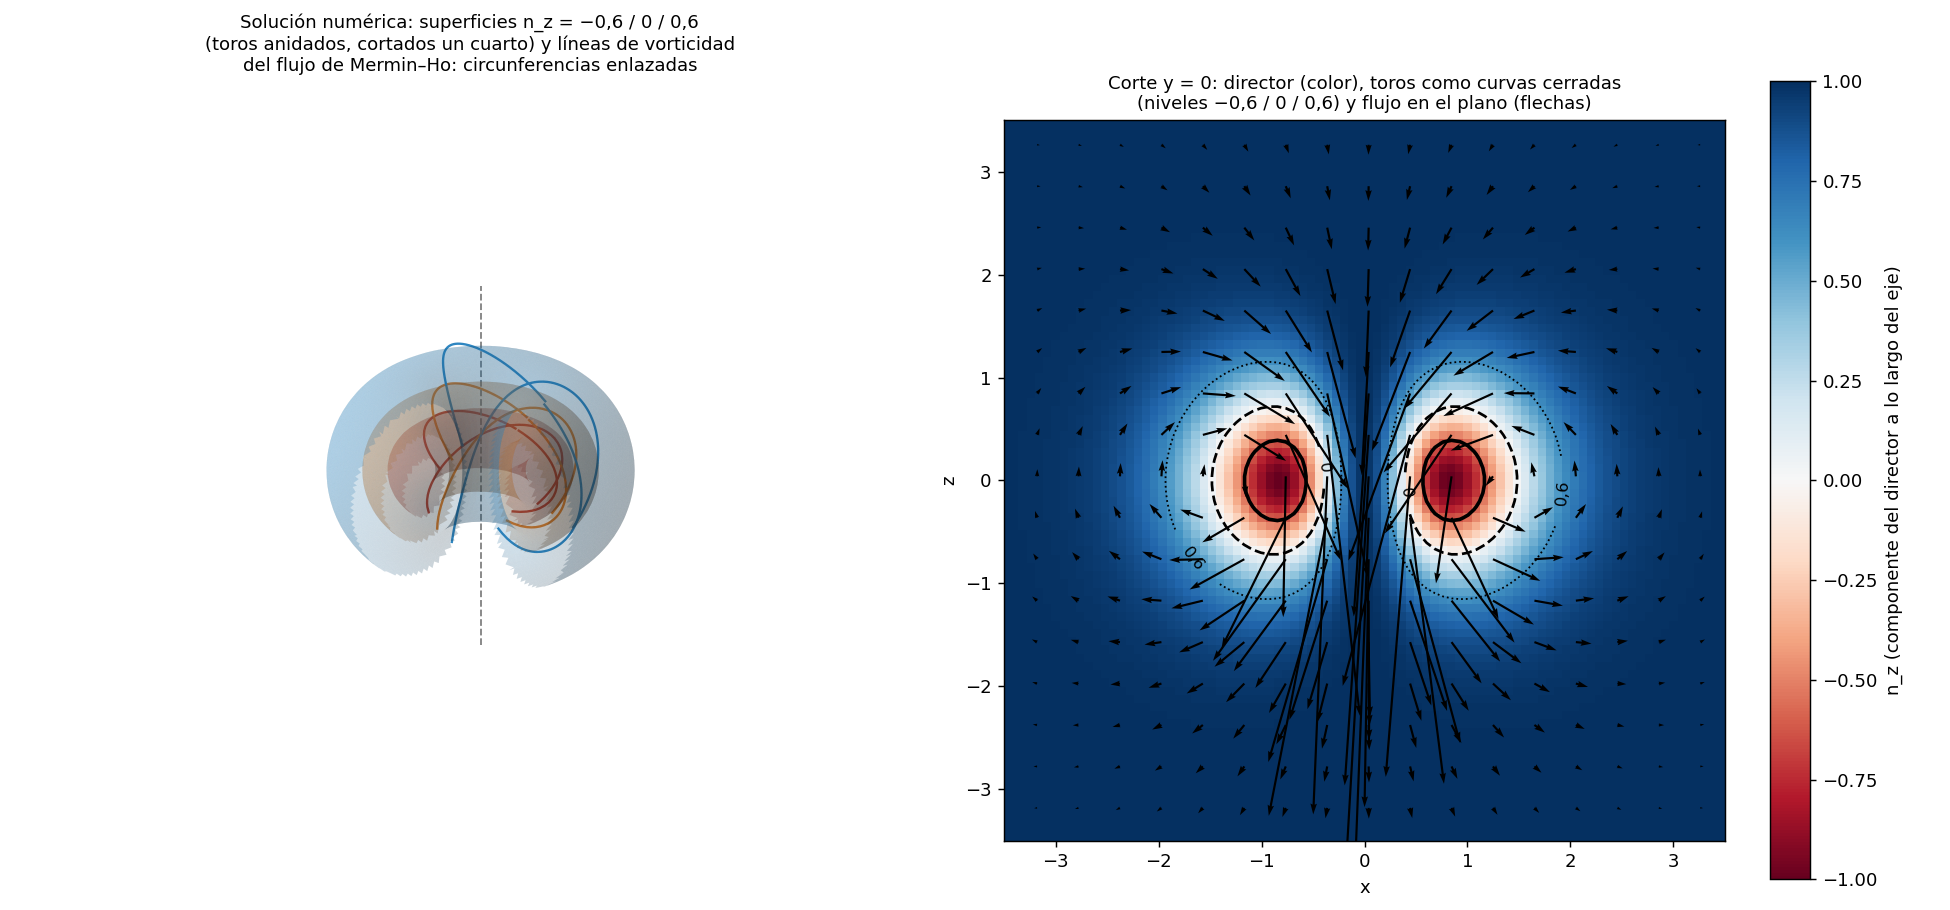
\includegraphics[width=\textwidth]{fig09_hopfion_k1.png}
\caption[El mismo hopfión con giro en $\eta$, $k=1$.]{El mismo hopfión con el giro en la dirección compacta $\eta$ ($k=1$, misma malla, caja y escala que la figura~\ref{fig:hopf-k0}). El giro es una rotación global alrededor de $\hat{\vb{z}}$ en cada corte de $\eta$, así que $n_z$, la vorticidad y el flujo no dependen de $\eta$ y la figura vale para cualquier corte. Comparada con $k=0$, el anillo se contrae (radio del núcleo $0,835$ frente a $1,184$) y el director vuelve al reposo mucho antes. Lejos del anillo, el giro añade a la energía el término $k^2|\vb{n}_\perp|^2$, y la ecuación linealizada es la de Poisson apantallada, $-\nabla^2\vb{n}_\perp+k^2\vb{n}_\perp=0$ (la misma del apantallamiento de Debye): la cola debe ser $1-n_z\sim e^{-2kr}/r^2$, con alcance $1/k$ \st{D}. El ajuste numérico de la cola da $k_{\mathrm{ef}}=1,064$ para $k=1$ (6~\%) \st{N}. Para $k=0,5$ y $k=0$ la caja de lado~12 contamina la cola (sin giro aparece un $k_{\mathrm{ef}}=0,37$ espurio, efecto de la pared), así que esos dos casos no sirven todavía como comprobación \st{A}.\par\smallskip
\emph{Nota:} esta figura ilustra el efecto del giro. Si el nudo es el ancla del leptón, mucho menor que la longitud de Compton ($k\ll1$; sección~5, punto~8), el aspecto del electrón es el de la figura~\ref{fig:hopf-k0}, como confirma el cálculo con $k=0,1$. Elaborada con \prog{figura\_hopfion.py}.}
\label{fig:hopf-k1}
\end{figure}

\apartado{Forma de la cola} (\prog{cola\_angular.py}). Lejos del anillo, la desviación del director $n_\perp=n_x+i\,n_y$ tiene simetría axial alrededor del eje del nudo y perfil dipolar, $|n_\perp|^2\propto\operatorname{sen}^2\theta$ ($\theta$ medido desde el eje): nula sobre el eje y máxima en el ecuador. Medida en capas esféricas entre $r\approx2$ y~4 \st{N}: con $k=0$ y $k=0,1$, el cociente de Legendre $a_2/a_0$ vale $-1,00\pm0,015$ desde $r\approx3$ ($\operatorname{sen}^2\theta$ puro da $-1$), sin términos impares. Con $k=1$ toda la ventana queda más allá de $1/k$; aparece además un octupolo de un 0,8~\% en amplitud, y su proporción respecto al dipolo sigue exactamente el cociente $k_3(kr)/k_1(kr)$ de la ecuación lineal con masa (constante, $0,0083\pm0,0003$, desde $r\approx3$). Es lo esperado \st{D}: entre el núcleo y $1/k$ el campo se comporta como sin masa y los multipolos altos se borran (el octupolo como $(\ell/r)^2$ respecto al dipolo); más allá de $1/k$ todos decaen como $e^{-kr}/r$ y la forma queda congelada. Con $k=1$ no hay zona intermedia, porque $1/k$ es del orden del núcleo. En el caso del ancla ($k\ll1$) el octupolo llegaría a la cola reducido en un factor $(\ell/\lbar_C)^2$ y el halo sería dipolar casi puro, alineado con el eje del nudo \st{H, extrapolación de la misma ecuación, no simulada}. Control: en la solución con $k=1$ el virial se desvía un 4,8~\% (un 1,8~\% sin giro), efecto de la resolución (unos 10 puntos por radio del anillo); no cambia la forma de la cola, pero la cifra del octupolo es aproximada \st{A}.

\begin{figure}[!htb]
\centering
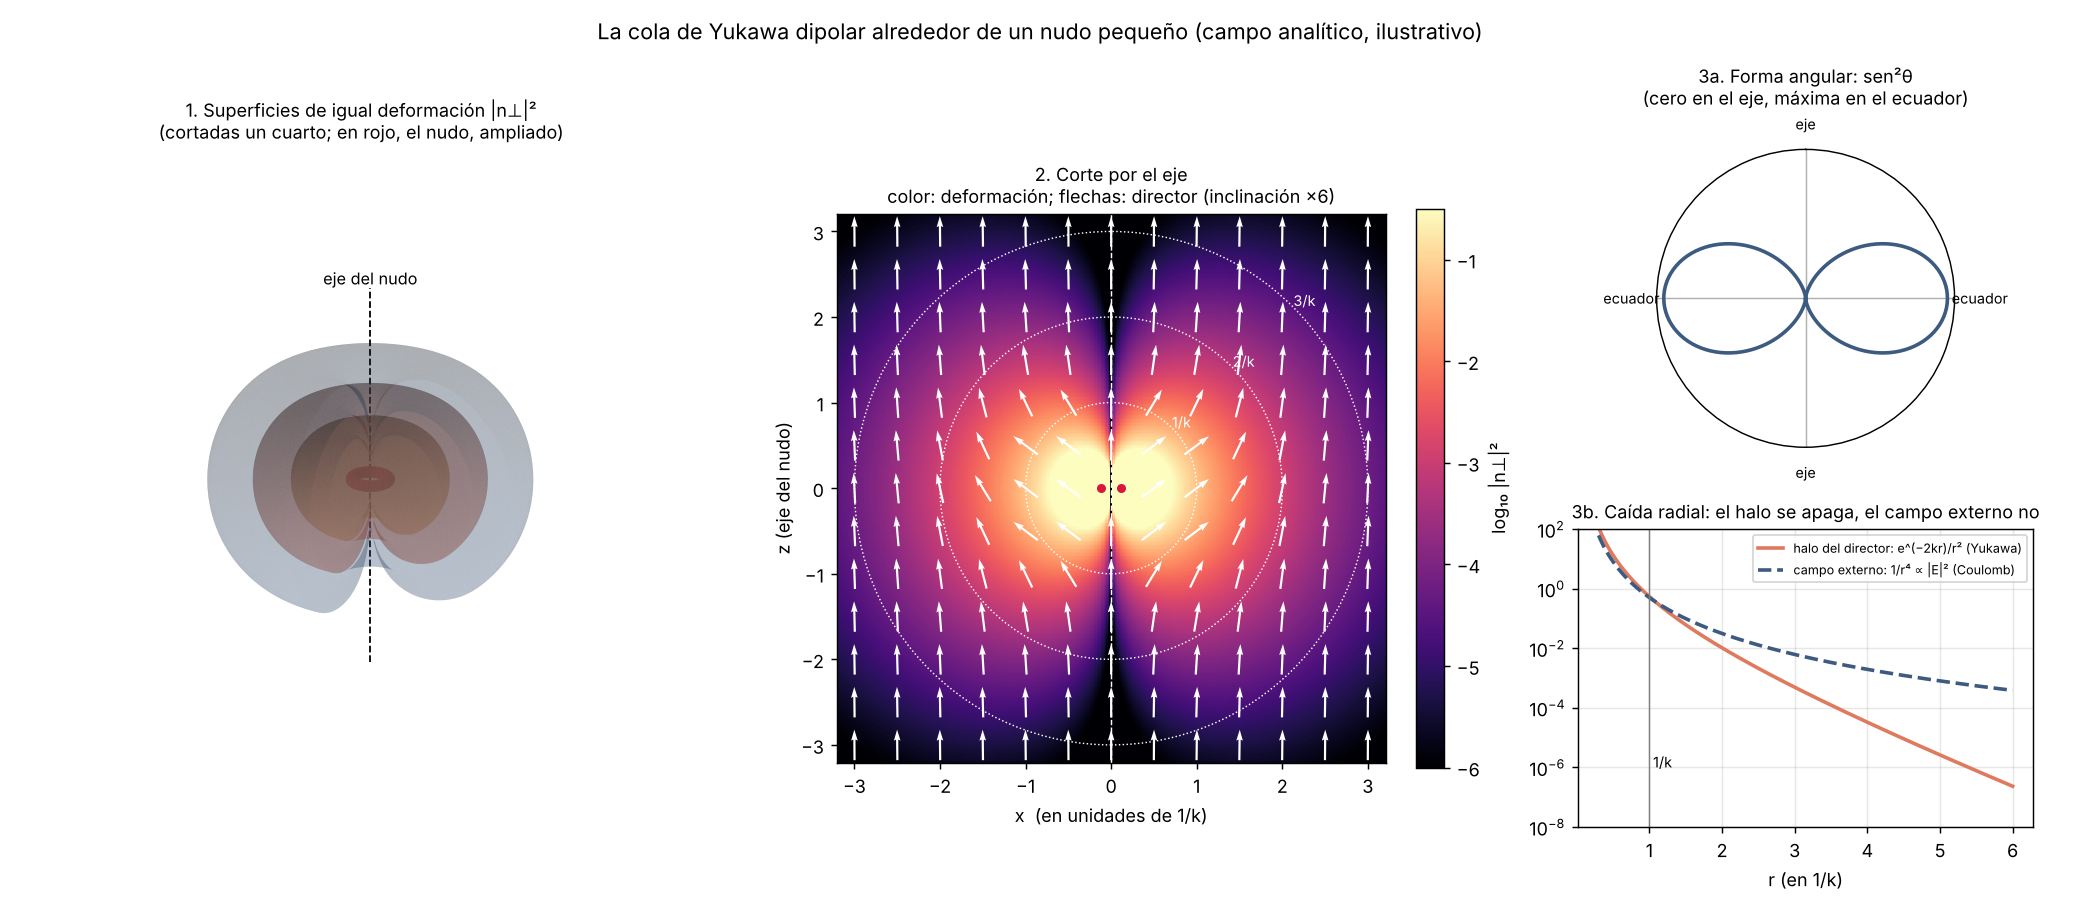
\includegraphics[width=\textwidth]{fig10_cola_dipolar.png}
\caption{La cola de Yukawa dipolar alrededor de un nudo pequeño. Es el campo analítico $n_\perp\propto(x+iy)\,k_1(kr)$, no la simulación; las medidas del apartado «Forma de la cola» muestran que la simulación tiene esta forma. Distancias en unidades de $1/k$ ($\lbar_C$ si $k=1/\lbar_C$). 1:~superficies de igual deformación $|n_\perp|^2$, cortadas un cuarto: manzanas alrededor del eje, con un hoyuelo en cada polo; el nudo, en rojo, dibujado mayor de lo que es para que se vea. 2:~corte por el eje; el color es la deformación (escala logarítmica) y las flechas el director, con la inclinación multiplicada por~6: lejos apunta al reposo, cerca del nudo se abre hacia fuera en el ecuador y no se abre a lo largo del eje. Con el giro en $\eta$ la dirección en que se abren las flechas rota alrededor del eje al recorrer $\eta$; la intensidad no cambia. 3a:~la forma angular, $\operatorname{sen}^2\theta$. 3b:~caída con la distancia; hasta $1/k$ el halo y el campo de Coulomb caen de forma parecida, después el halo se apaga exponencialmente. La figura muestra de dónde saldría la orientación del momento magnético (el eje del nudo), no su valor (sección~5, punto~8). Elaborada con \prog{figura\_cola\_dipolar.py}.}
\label{fig:cola}
\end{figure}

\apartado{Espín $+\tfrac12$ y $-\tfrac12$ en el flujo.} Pasar de $+\tfrac12$ a $-\tfrac12$ es dar la vuelta al nudo: girarlo $180^\circ$ alrededor de un eje perpendicular al suyo. Vistas desde fuera, todas las líneas de flujo invierten su sentido, el chorro del eje y el enroscado alrededor de él, pero el enlace entre ellas y la carga de Hopf no cambian: es el mismo objeto orientado al revés \st{D}. La imagen especular es otra cosa: invierte solo el enroscado, conserva el sentido del chorro y cambia el signo del enlace; es un nudo de rosca contraria, no un cambio de espín \st{D}. Qué partícula le correspondería es una pregunta abierta \st{A}; en el modelo el signo de la carga es el sentido de circulación en $\eta$, no el signo de $Q$. Coherencia con el plano compacto \st{H}: dar la vuelta al nudo es un giro de $180^\circ$ en las extendidas, y un espinor gira la mitad, de modo que su fase cambia $90^\circ$; en el plano compacto, las líneas que unen las nucleaciones de los dos estados de espín son perpendiculares ($90^\circ$). La regla de la mitad del ángulo enlaza las dos imágenes; no se ha calculado como tal.

\begin{figure}[!htb]
\centering
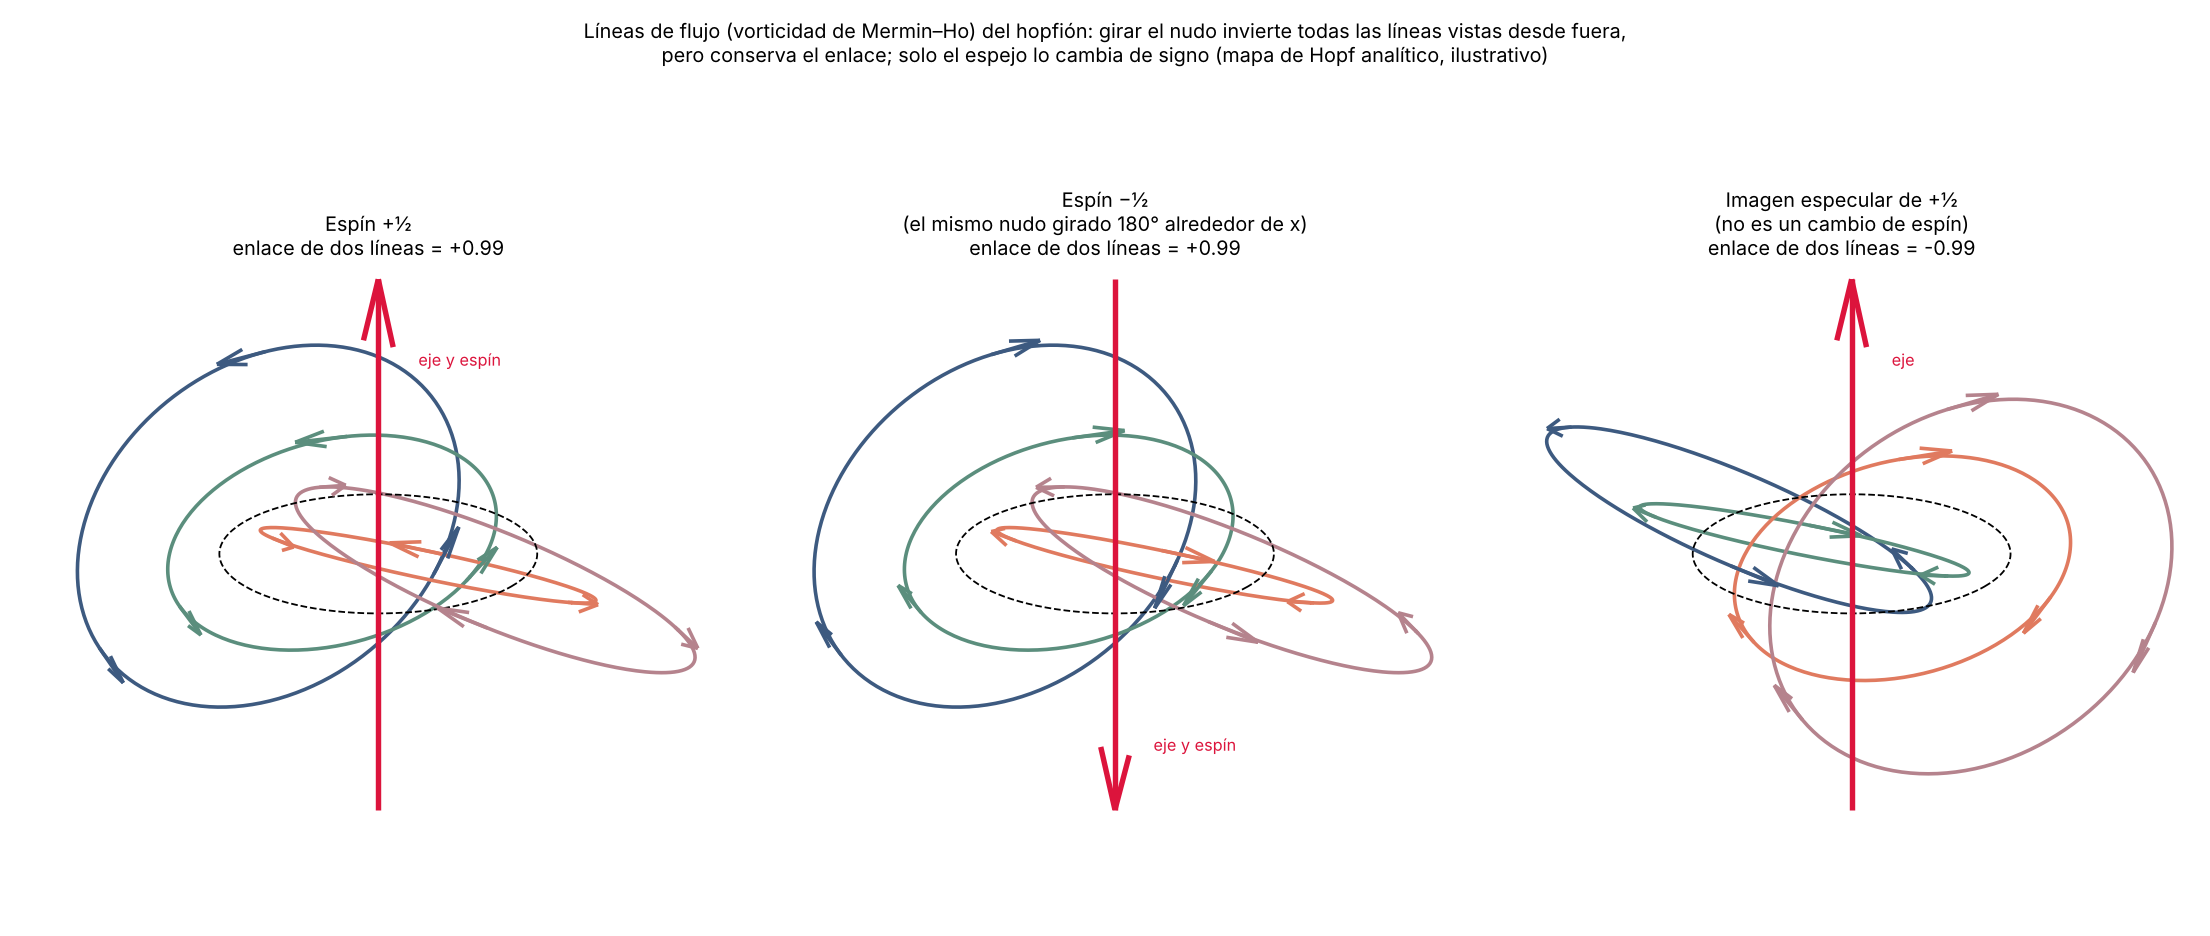
\includegraphics[width=\textwidth]{fig11_espin_flujo.png}
\caption{Líneas de vorticidad del flujo de Mermin--Ho de un hopfión analítico (mapa de Hopf de carga~1, ilustrativo, no la simulación); en línea discontinua, el núcleo del anillo; en rojo, el sentido del chorro sobre el eje. Izquierda: espín $+\tfrac12$. Centro: espín $-\tfrac12$, el mismo nudo girado $180^\circ$ alrededor de $x$; las líneas pasan por los mismos sitios en sentido contrario y el enlace de dos de ellas sigue siendo $+1$ (calculado con la integral de Gauss: $+0,99$). Derecha: imagen especular de $+\tfrac12$ ($z\to-z$); el chorro no cambia, el enroscado sí, y el enlace pasa a $-1$ ($-0,99$). Elaborada con \prog{figura\_espin\_flujo.py}.}
\label{fig:espin-flujo}
\end{figure}

\apartado{Giro en $\eta$.} Con $\vb{n}(\vb{x},\eta)=R_{\hat{z}}(k\eta)\,\vb{n}_3(\vb{x})$, el problema se reduce exactamente a 3D con un término de masa $k^2\!\int(1-n_z^2)$ y otro $k^2\!\int|\nabla n_z|^2$. Malla $150^3$, caja~12:

\begin{center}
\small
\begin{tabular}{@{}ccccc@{}}
\toprule
$k$ & Energía & $\Delta E$ & $\Delta E/k^2$ & $Q$ \\
\midrule
0   & 544,35 & ---   & ---  & $-0,979$ \\
0,5 & 586,68 & 42,3  & 169  & $-0,973$ \\
1   & 675,38 & 131,0 & 131  & $-0,959$ \\
\bottomrule
\end{tabular}
\end{center}

A primer orden en $k$ la masa añadida es $k^2I_0$, con $I_0\approx168$ la integral del hopfión sin giro; el valor medido con $k=0,5$ (169) coincide. Con $k=1$ el giro comprime el nudo y el cociente baja.

\apartado{Giro pequeño ($k=0,1$).} Arrancando de la solución de $k=0$, misma malla y caja: $E=545,98$, es decir $\Delta E\approx1,6$ frente a $k^2I_0\approx1,7$ \st{N}. El perfil del director es prácticamente el de $k=0$ (radio del núcleo $1,162$ frente a $1,184$), así que con $k\ll1$, que es el caso de un nudo mucho menor que la longitud de Compton, el aspecto del hopfión es el de la figura~\ref{fig:hopf-k0}. Cautela: tras 10\,000 iteraciones la energía seguía bajando muy despacio y el virial se desviaba de cero; parte de la pequeña contracción del radio se debe a esa relajación y a la caja, no al giro (a primer orden en $k^2$ se esperaría solo un 0,3~\%). Con este giro la cola no se puede medir en la caja de lado~12.

\apartado{Limitación declarada: giros grandes ($k\geq2$) \st{A}.} Con $k=2$ el nudo se contrae por debajo de lo que resuelven nuestras mallas ($h=0,06$ en caja de lado~6): la energía baja de 544 y la carga de Hopf pasa a~0. Es un defecto numérico, no físico \st{D}: los dos términos del giro son positivos, así que un nudo con $Q=1$ nunca puede tener con giro menos energía que sin él (544), y en el continuo la carga no puede desaparecer. Resolverlo exigiría mallas de $h\approx0,03$ o derivadas de cuarto orden. Esa misma cota sirve de control en cualquier cálculo con giro: si $E$ baja de 544, el nudo se ha perdido. Además, a nudos pequeños el término de cuarto orden obliga a pasos de tiempo mucho menores; \prog{hopfion\_eta.cpp} los reduce solo cuando la energía sube.

\apartado{Estabilidad.} Las soluciones son mínimos locales de la energía (flujo de gradiente), luego estables frente a perturbaciones pequeñas que respetan la forma del giro (Lagrange--Dirichlet).

\apartado{Liberación de la energía del nudo: aniquilación.} Mientras $Q=1$ la energía no puede bajar del mínimo: toda deformación continua conserva $Q$, y existe una cota inferior $E\geq c\,|Q|^{3/4}$ (Vakulenko y Kapitanskii, 1979) \st{D}. Solo hay dos formas de liberarla. (1)~Deshacer el nudo en un punto donde el director quede indefinido, es decir, fundiendo localmente el orden (un núcleo de fase isótropa); ese núcleo cuesta energía, así que hay una barrera y el nudo no se deshace solo \st{D sobre la topología; H sobre la fase}. (2)~Encontrarse con un nudo de carga opuesta, $Q=-1$: la carga total es~0, el conjunto puede deshacerse de forma continua y se libera toda la energía de ambos. Es la imagen de la aniquilación de partícula y antipartícula, sin mecanismo añadido \st{H}. El electrón y el positrón viven en la misma interfaz entre las dos fases esmécticas en la que se propaga el fotón, una corriente transversal libre sin estructura en las compactadas ($k=0$). Al deshacerse el nudo, la energía pasa, por la no linealidad del sustrato, del modo confinado $\pm\tfrac12$ al modo libre de esa misma interfaz: a fotones, al menos dos por conservación del impulso \st{H}.

% =====================================================================
\section{Lo descartado}

Siete vías probadas y descartadas, cada una con su razón; delimitan qué necesita el modelo.

\begin{center}
\small
\begin{tabularx}{\textwidth}{@{}Y Y Y@{}}
\toprule
Vía & Resultado & Razón \\
\midrule
Solitón escalar con umbral, frecuencia libre & Cae a estados con autoenlace ($\omega\approx0,88$) & Contradice el postulado de energía de autoenlace nula \\
\addlinespace
Solitón escalar con frecuencia anclada & Núcleo crítico: se disuelve o la meseta invade el espacio & Teorema de Derrick \\
\addlinespace
Término de cuarto orden sin topología & Sigue inestable & Frena el cambio de tamaño, no la caída de amplitud; Skyrme funciona por la topología \\
\addlinespace
Giro en un solo plano de las extendidas & Anillo con autoenlace (frecuencia libre) o invasión (anclada) & Sin cantidad conservada, Derrick sigue mandando \\
\addlinespace
Quiralidad en lugar del cuarto orden & El nudo se deshace ($q=\pm0,8$, $k=1$) & Haría falta $q/k\approx20$, pero con $q>k$ el estado uniforme se vuelve hélice \\
\addlinespace
Giro del director en el tiempo, a momento angular fijo, en lugar del cuarto orden & El giro se acelera hasta $\omega\approx1,7>k$ y el nudo se deshace ($Q$ de $-0,97$ a~0; $c_4=0$, $k=1$) & Virial: el equilibrio exige $\omega^2=k^2+E_2/(3I)>k^2$, y entonces la cola radia; el mecanismo de Volovik y Mineev usa momento de traslación \\
\addlinespace
Estructura compacta (anchura, forma) como origen de $g-2$ & $g=2$ exacto & En Foldy--Wouthuysen el término lineal solo usa la carga media del modo más bajo \\
\bottomrule
\end{tabularx}
\end{center}

\apartado{Restricción que deja la quiralidad \st{D}.} Un término quiral en la energía da masas distintas a cargas de Hopf $+1$ y $-1$, es decir, a partícula y antipartícula, lo que contradice la igualdad de masas de electrón y positrón. En el sector del electrón debe ser despreciable.

\apartado{Errores corregidos durante el trabajo.} Un cálculo de $g$ con un director (vector) que gira dio primero $g=2$ por omitir el factor~2 de las densidades de impulso canónicas; el valor correcto es $g=1$ (orbital). Es lo que llevó a la ecuación espinorial.
% =====================================================================
\section{Lo abierto}

Trece problemas sin resolver; el primero decide si el modelo explica la anomalía o solo el valor base $g=2$.

\begin{enumerate}[label=\arabic*.,leftmargin=*]

\item \textbf{La anomalía $g-2=0,00116$.} Vía más prometedora \st{H}: el arrastre propio no cambia la trayectoria de la pulsación pero sí su velocidad efectiva, como el medio que arrastra la luz en el experimento de Fizeau. Si entra en la corriente de carga y no en la masa ni en el espín, $a=v_a/c$, con $v_a\propto\alpha$. Falta calcular $v_a$ a partir del acoplamiento de Coulomb y ver si la geometría da el $2\pi$. Otra fuente posible: la textura del nudo en las extendidas (corriente orbital con $g=1$). Conexión posible con el postulado~6 \st{H, especulativa}: en un medio que gira, el plano de polarización de la luz es arrastrado en $(n_g-1/n_\varphi)\,\Omega/c$ por unidad de longitud, que se anula para $n=1$ (Player, 1976; Jones, 1976; Götte, Barnett y Padgett, 2007). Si la pulsación ve el hyle con índice~1, su marco no sigue la vorticidad del arrastre (marco anclado, $g=2$); si el arrastre propio aparta su velocidad efectiva de $c$, el anclaje deja de ser perfecto y $g$ se separa de~2. El marco anclado y la anomalía serían entonces el mismo efecto. Plan: (1)~calcular $c_1$ en $a=c_1\,v_a/c$ con la ecuación espinorial; (2)~calcular $c_2$ en $v_a/c=c_2\,\alpha$ a partir de la circulación cuantizada en $\eta$ y de la respuesta del hyle; (3)~comprobar $c_1c_2=1/2\pi$ (Schwinger). Advertencia de circularidad: usar el valor medido de $a$ para obtener $v_a$ y de ahí $\alpha$ no predice $\alpha$, solo comprueba el coeficiente $1/2\pi$; $\alpha$ solo quedaría predicha si $v_a$ se calcula sin introducir $e$ ni $a$.

\item \textbf{El marco anclado a las capas (postulado~6).} El postulado tiene una motivación mecánica: el cilindro es intrínsecamente plano y la permeación nula y la alta viscosidad en $\xi$ impiden que las capas se inclinen. Queda por demostrar \st{A}: (i)~con la elasticidad del esméctico (módulos $B$ y $K$), que el arrastre en $\eta$ no retuerce las capas; (ii)~que la métrica efectiva de Unruh desvía la trayectoria sin girar el marco.

\item \textbf{Unir el espinor y el nudo:} escribir el director como bilineal del espinor (Hopf) y comprobar que el hopfión sigue saliendo con el espín cuantizado a $\hbar/2$. Condición que debe cumplir \st{D}: el espinor va como $e^{i\eta/2}$, pero el director es un vector y tiene que volver a ser el mismo tras una vuelta en $\eta$; al construirlo como bilineal sus fases se duplican, de modo que su giro es el doble que el del espinor ($k_{\mathrm{director}}=2\,k_{\mathrm{espinor}}$). Tras una vuelta en $\eta$ el toro ha girado una vuelta completa alrededor de su eje y vuelve a ser el mismo, mientras que el espinor ha cambiado de signo. Por la simetría del hopfión de carga~1, avanzar en $\eta$ equivale a girar el toro alrededor de su propio eje, sin precesión; la precesión del eje solo la produce un campo externo (frecuencia de Larmor). La imagen de Ohanian como proyección \st{H}: la circulación de la densidad de momento de la onda de Dirac alrededor del eje del espín (Ohanian, 1986) sería la proyección en las tres extendidas de la pulsación con su nudo. Lo que circula en $\eta$ se vería en las extendidas como el flujo toroidal del hopfión alrededor de su eje. Falta comprobar que, con el director escrito como bilineal del espinor, ese flujo dé el momento angular $\hbar/2$ y no solo su orientación: el cálculo con el director solo da $g=1$ (sección~4). Qué es el director del nudo \st{H}. El director del hopfión vive en las extendidas, mientras que la normal a las capas es la dirección $\xi$, dentro del plano compacto. Propuesta: el director es una dirección en las cinco dimensiones espaciales; en el esméctico~A coincide con la normal $\xi$, y en \Cst{} se inclina respecto a ella. La dirección de esa inclinación hacia las extendidas es un vector unitario en tres dimensiones, y ese sería el campo cuya textura forma el nudo. Dos consecuencias: (i)~sin inclinación no hay nudo, así que el hopfión solo puede existir donde la hay; (ii)~junto a la interfaz A/\Cst{} la inclinación es pequeña (postulado~4), y la textura solo necesita que su dirección esté definida, pero la rigidez $\kappa_2$ y la energía del nudo crecerían con la inclinación \st{A}.

\item \textbf{Estabilidad frente a perturbaciones que rompen la forma del giro en $\eta$:} requiere un cálculo en 4D $(x,y,z,\eta)$.

\item \textbf{Fijar la escala $\ell=\sqrt{\kappa_4/\kappa_2}$.} Las rigideces $\kappa_2$ y $\kappa_4$ no se han derivado del sustrato, así que el tamaño del hopfión no tiene todavía valor en metros \st{A}. Hipótesis para fijarlo \st{H}: el giro del hopfión en $\eta$ es el mismo que el del espinor, $k=\tfrac12/\xi_0=mc/\hbar$; entonces $k_{\mathrm{programa}}=\ell/\lbar_C$ ($\lbar_C$, longitud de Compton reducida). Los cálculos con $k=1$ ($\ell=\lbar_C$: anillo de $0,835\,\lbar_C\approx3,2\times10^{-13}$~m, alcance de la deformación $\lbar_C$) son un valor de prueba para estudiar el efecto del giro, no «el electrón»: la hipótesis del ancla (punto~8) exige $\ell\ll\lbar_C$, es decir $k\ll1$, como en el cálculo con $k=0,1$. Falta una segunda condición que lo cierre: que la energía del hopfión ($\approx544\sqrt{\kappa_2\kappa_4}$ cuando $k\ll1$) sea compatible con $mc^2$, y un argumento que fije $\ell/\lbar_C$.

Hipótesis alternativa: $\ell$ del orden del radio clásico \st{H}. Si $\ell\approx r_e=\alpha\,\lbar_C\approx2,8\times10^{-15}$~m, el nudo del electrón es un ancla ($k=\alpha\approx0,007$, prácticamente sin contraer), $\alpha$ aparece en la geometría ($\ell/\lbar_C=\alpha$; compárese con $a=\alpha/2\pi$ del punto~1, todavía sin mecanismo) y el halo es dipolar casi puro (el octupolo se reduce en un factor $\alpha^2$). El choque explora el electrón de fuera adentro: primero el campo (dispersión de Rutherford/Mott), luego la envolvente y el halo, a la escala $\lbar_C$ (el paso de Thomson a Klein--Nishina, que el modelo tiene que reproducir), y por último el nudo. Para el nudo, el límite experimental (en la dispersión de Bhabha a 130--207~GeV la escala de interacciones de contacto supera 15--27~TeV, Xi, Liu y Ulbricht, 2024, lo que equivale a unos $10^{-20}$~m) se salvaría si el nudo es blando: al encogerlo un factor $\lambda$ su energía va como $E_2\lambda+E_4/\lambda$ \st{D}, así que un choque de energía $E$ puede comprimirlo hasta $s\approx\ell\,E_{\mathrm{nudo}}/(2E)$. Con $\ell\approx r_e$ y $E_{\mathrm{nudo}}\lesssim m_ec^2$, $s\lesssim(\alpha/2)\,\hbar c/E$: el nudo comprimido sería siempre unas 270 veces menor que la resolución de la sonda, a cualquier energía (con $E=100$~GeV, $s\approx10^{-20}$~m). Problemas abiertos \st{A}: (i)~si el nudo tiene tiempo de comprimirse durante el choque: falta comparar su tiempo de respuesta con la duración del choque; (ii)~$E_{\mathrm{nudo}}\lesssim m_ec^2$ es una suposición, que fija $\sqrt{\kappa_2\kappa_4}$; (iii)~un objeto de tamaño $(\alpha/2)\,\hbar c/E$ deja en el factor de forma una huella relativa del orden de $(\alpha/2)^2\approx10^{-5}$, que habría que contrastar con el momento magnético, medido con unas 13 cifras; (iv)~la carga tiene que estar en el nudo en el momento del choque (punto~8). Si $\ell$ es una propiedad del medio, $k=\ell/\lbar$ valdría $\approx1,5$ para el muón y $\approx25$ para el tauón, más allá de lo que resuelven nuestras mallas; no se aplica si muón y tauón son excitaciones del electrón (punto~10). Tal como está, la imagen en capas reproduce lo que se mide pero no da observables nuevos; la única puerta sería el halo del director, si alguna sonda se acopla a él. Un indicio a favor de esta hipótesis frente a $\ell\approx\lbar_C$: que dos electrones no se fundan exige $\ell\lesssim3\,r_e$ (punto~6).

\item \textbf{Por qué no se funden dos electrones.} En la energía de Faddeev--Skyrme dos nudos de $Q=1$ que se funden en uno de $Q=2$ liberan energía: con $E\propto Q^{3/4}$, del orden del 18~\% de la masa en reposo (estimación de escala; Sutcliffe, 2007). Un objeto estable con carga $2e$ y unas $1,6\,m_e$ se habría observado, así que la fusión tiene que estar prohibida en el vacío \st{D + dato experimental}. Lo que debería impedirla no está en la energía del director: la repulsión por el arrastre en $\eta$ y la exclusión de los espinores. Estimación de la repulsión \st{H}: si la carga está donde está el nudo (punto~8), fundir dos cargas $e$ en un objeto de tamaño $\ell$ cuesta unos $2k\,e^2/(4\pi\varepsilon_0\ell)=2k\,mc^2\,(r_e/\ell)$, con $k$ entre $\tfrac12$ y $\tfrac35$ según el reparto de la carga, mientras que la fusión libera unos $0,36\,mc^2$ si la energía del nudo es $\approx mc^2$. Con $\ell\approx r_e$ el coste ($\approx mc^2$) es casi el triple de la ganancia: el nudo fundido tendría más energía que los dos separados, así que la fusión está prohibida y no solo frenada por una barrera. La prohibición se mantiene mientras $\ell\lesssim3\,r_e$: es una cota superior al tamaño del nudo, y un indicio a favor de un nudo pequeño (con $\ell\approx\lbar_C$, unas $137\,r_e$, los nudos sí se fundirían). Depende de dos supuestos ya declarados: que la carga esté en el nudo y que $E_{\mathrm{nudo}}\approx mc^2$ (punto~5, ii). Falta el cálculo de la exclusión \st{A}. (No es el par de Cooper: este tiene enlace de meV, tamaño de 100~nm a 1~$\mu$m y solo existe en un sólido; en el modelo sería, en todo caso, dos nudos $Q=1$ débilmente ligados a distancia, sin fundirse \st{H}.)

\item \textbf{Condiciones que el modelo debe cumplir.} No son postulados sino pruebas que el modelo tiene que superar. (a)~\emph{Paso de leptón aislado a orbital sin energía suplementaria:} al ligarse, el nudo no se deshace y no se libera más energía que la de enlace del átomo. (b)~\emph{La estructura descrita no se observa:} en las colisiones el electrón se comporta como puntual hasta unos $10^{-18}$~m o menos, mientras que el nudo tiene un tamaño $\ell$ todavía sin fijar (punto~5): unos $3\times10^{-13}$~m si $\ell\approx\lbar_C$, y unos $3\times10^{-15}$~m si $\ell\approx r_e$; para el segundo caso, el punto~5 propone que el choque comprime el nudo por debajo de la resolución de la sonda. Tensión declarada \st{A}: en la energía del director los términos escalan como $\lambda$, $1/\lambda$ y $\lambda^3$ con el tamaño $\lambda$ del nudo, así que un nudo extendido hasta el tamaño de un orbital costaría muchísima energía. La lectura compatible con (a) es que el nudo conserva su tamaño y que el orbital es la envolvente, que describe el estado del leptón; la envolvente del leptón no tiene coordenada interna. Para (b), lo que miden las colisiones, la distribución de carga, no puede seguir la forma del nudo; la carga viene de la circulación en $\eta$, fijada por la interfaz A/\Cst, y no del director. El argumento es la universalidad: la carga es idéntica en todas las partículas cargadas (la del electrón y la del protón coinciden en valor absoluto con una precisión mejor que una parte en $10^{21}$), y eso solo puede salir de un rasgo geométrico fijo como una interfaz, no de una textura cuyo tamaño y energía cambian con el estado \st{D, dado el postulado~5}. Esto separa el valor de la carga del nudo: el valor lo fija la interfaz y la posición la marca el nudo. La distribución $|\Psi|^2$ es la probabilidad de dónde está el nudo, y en un choque la carga entera está donde está el nudo (puntos 5 y~8). Lo que falta demostrar es lo otro: cómo se distribuye esa carga en las extendidas, es decir, que el factor de forma sea el de una carga puntual hasta momentos transferidos muy altos \st{A}.

\item \textbf{El nudo como ancla del leptón \st{H}.} Las ecuaciones de la envolvente son iguales en todos los puntos del espacio y nada en ellas dice dónde está un leptón aislado; el nudo del director, estable y con centro, puede hacer de ancla. Imagen de un orbital~s: dos cosas a la vez. El torbellino en $\eta$ llena el orbital, repartido como $|\Psi|^2$, y da una densidad de carga continua; el nudo, pequeño, se mueve libre por el orbital, con probabilidad $|\Psi|^2$ de encontrarlo en cada sitio. Así el orbital no exige expandir el nudo (condición~(a) del punto~7). Precedentes: la carga como $e|\Psi|^2$ es la interpretación original de Schrödinger (1926), abandonada porque la nube se repelería a sí misma; aquí no ocurriría si la carga entera está donde está el nudo y $|\Psi|^2$ es la probabilidad de encontrarlo \st{H; punto~7}, y un campo simétrico no empuja a su fuente (postulado~8). Un centro que se mueve de forma irregular con distribución $|\Psi|^2$ es la mecánica estocástica de Nelson (1966); el ruido podrían darlo las fluctuaciones del hyle cerca del punto tricrítico. Exigencias y problemas abiertos \st{A}: (i)~si las colisiones golpean el nudo, tiene que parecer puntual, lo que obliga a $\ell\ll\lbar_C$; (ii)~falta la ley que guía el nudo dentro de la envolvente; (iii)~hay que explicar por qué un detector encuentra siempre la carga entera en un punto (el problema de la medida en el modelo); (iv)~con dos partículas entrelazadas, el movimiento de cada nudo dependería del otro, como ya señaló Nelson para su teoría. Si el nudo sigue exactamente la distribución $|\Psi|^2$, el resultado es indistinguible de la mecánica cuántica estándar; el modelo ganaría una imagen física de lo que es una partícula, no observables nuevos.

Imagen del electrón en tres partes \st{H}. (1)~El nudo, pequeño: la topología y un eje. (2)~El halo del director, de alcance $1/k$ ($\lbar_C$ si $k=1/\lbar_C$), dipolar y alineado con ese eje (sección~3, «Forma de la cola»); es de corto alcance, porque decae exponencialmente, y no puede ser el campo eléctrico. (3)~Lejos, la onda estacionaria esférica de la envolvente, $\Psi\sim\operatorname{sen}(kr)/r$: su efecto promediado, proporcional a $|\Psi|^2$ (postulado~8), daría un campo estacionario con una parte esférica que cae como $1/r^2$ (la carga) y una parte dipolar que cae como $1/r^3$ (el momento magnético). Si ese dipolo comparte eje con el halo, el nudo sería lo que orienta el momento magnético, y la imagen del electrón quedaría cerrada en lo conceptual. Problemas abiertos \st{A}: (v)~en una onda puramente estacionaria el arrastre de Stokes neto se anula, así que el flujo medio necesita otra fuente: capas límite viscosas, como en el streaming de Rayleigh, o la rotación en $\eta$, que daría precisamente la parte dipolar; está sin calcular. (vi)~La circulación exterior debe dar el valor $e\hbar/2m$, con $g=2$; el nudo solo puede orientar el momento, no fijar su valor, que no puede depender de $\ell$.

\item \textbf{Dimensiones compactas de micras y límites experimentales.} Con $R_u\approx3,26~\mu$m las dos dimensiones compactas son «grandes» en el sentido de los modelos de dimensiones extra. (i)~La ley de la gravedad se ha comprobado hasta unas 50~$\mu$m con balanzas de torsión (grupo Eöt-Wash; Lee et al., 2020); 3~$\mu$m queda por debajo y no hay conflicto directo. (ii)~En los modelos de Arkani-Hamed, Dimopoulos y Dvali, donde la gravedad se propaga por las dimensiones extra, dos dimensiones de radio mayor que 0,66~$\mu$m quedan excluidas por el enfriamiento de la supernova SN~1987A (Hanhart et al., 2001), y las estrellas de neutrones dan cotas aún más estrictas. Esos límites salen de la emisión de gravitones de Kaluza--Klein; en el modelo la gravedad es un cambio del índice de refracción del hyle, no un gravitón que se propague por las compactadas, así que no se aplican directamente. (iii)~Una dimensión compacta de radio $R_u$ tiene modos con energías del orden de $\hbar c/R_u\approx0,06$~eV. En el modelo los más ligeros son los neutrinos ligeros (tipo~I), partículas conocidas que las estrellas emiten en abundancia, como se observa; no son estados nuevos \st{D dentro del modelo}. En una dimensión compacta ordinaria habría además una escalera de modos que una supernova produciría en enorme número. La escalera radial no existe, porque sus modos superiores son los que tienen nodos en $\xi$, y los nodos están prohibidos (postulado~1, apartado~2.0). La escalera angular, en $\eta$, depende del tipo de pulsación. Donde hay nucleaciones (electrón, $\nu_\tau$), el orden de Floquet solo está definido salvo múltiplos de~2: el orden $\tfrac32$ no es una familia nueva sino el segundo nivel de la de orden~$\tfrac12$, con el mismo espín~$\tfrac12$ y los mismos valores característicos \st{D, comprobado numéricamente con $q=0$, $-10$ y $-100$}. Sin potencial, ese nivel sería una circulación más rápida; con las nucleaciones es una vibración dentro de los pozos (véase el punto~10). Por eso no existen copias del electrón con espín~$\tfrac32$, como se observa. Queda abierto el caso de los neutrinos ligeros \st{A}: no tienen nucleaciones ($q\approx0$), así que sus órdenes superiores en $\eta$ serían circulaciones genuinas y ligeras; hay que comprobar que su acoplamiento o su masa los dejan fuera de los límites astrofísicos.

\item \textbf{Muón y tauón como modos de vibración de las nucleaciones \st{H}.} Las nucleaciones son ya otra fase del hyle, y pueden vibrar. Muón y tauón serían dos modos de vibración distintos que se activan sobre el electrón: uno de compresión de las capas y otro de abanico, cada uno controlado por un módulo de elasticidad distinto del esméctico (la rigidez de compresión $B$ y la de flexión o abanico $K$, en la notación de de~Gennes). Al depender de módulos distintos, sus masas no tienen por qué seguir una escalera regular, lo que es coherente con que la diferencia tauón--electrón sea unas 17 veces la diferencia muón--electrón, y no un múltiplo simple. Ambos tienen espín~$\tfrac12$ y viven en la misma interfaz A/\Cst, con la misma carga que el electrón. Que los modos dependan de las nucleaciones lo apoya un dato: no se ha observado ninguna partícula neutra de masa parecida. Las nucleaciones son los dos máximos de intensidad de la onda de orden~$\tfrac12$ que circula; sin circulación no hay nucleaciones, así que cualquier vibración suya va unida a una carga, y no puede existir un «muón neutro». Si la vibración es en $\xi$, explicaría además cómo se desintegran: el fotón y el campo eléctrico son corrientes paralelas a $\eta$, y una vibración en $\xi$ difícilmente se convierte en ellas, lo que suprimiría $\mu\to e\gamma$, prohibida experimentalmente con gran precisión; en cambio los neutrinos son perfiles radiales en $\xi$ (tipo~I), así que la vibración se acoplaría de forma natural a ellos, que es como decae el muón. Problemas abiertos \st{A}: (i)~calcular las frecuencias de los dos modos y relacionarlas con las masas; como las frecuencias van como la raíz cuadrada de los módulos, una vía es que sus cocientes sean cocientes universales del punto tricrítico, números puros que dependen solo del tipo de transición y no se ajustan; cualquier regla debe reproducir la relación empírica de Koide entre las tres masas,
\[
\frac{m_e+m_\mu+m_\tau}{\bigl(\sqrt{m_e}+\sqrt{m_\mu}+\sqrt{m_\tau}\bigr)^2}=\frac23 ,
\]
que se cumple con una precisión de 1 entre 100\,000; (ii)~convertir la regla de selección cualitativa de la desintegración en un cálculo del acoplamiento; (iii)~el neutrino tauónico también tiene nucleaciones ($q=-0,6393$), y no se han observado neutrinos pesados: hay que explicar por qué sus nucleaciones no tienen modos excitados observables, quizá porque los modos de compresión y abanico necesitan la interfaz A/\Cst{} y el tauónico vive dentro de \Cst, o porque con $|q|$ pequeño sus modos tienen energías o acoplamientos muy distintos.

\item \textbf{La imagen especular del nudo y el positrón} \st{H}. La imagen especular del hopfión tiene la rosca contraria (enlace $-1$; sección~3, figura~\ref{fig:espin-flujo}). Hipótesis: es el positrón, porque la circulación en $\eta$ y la de las extendidas están acopladas. Lo que exige \st{A}: (i)~un término que dependa del signo relativo de las dos circulaciones; la energía actual va como $k^2$ y no lo distingue \st{D}. Candidato: la helicidad cruzada de Moffatt de dos familias de tubos de vorticidad enlazados, $H=H_1+H_2+2L\,\Phi_1\Phi_2$, que en un medio sin disipación se conserva y bloquearía el signo relativo. (ii)~Con ese acoplamiento, electrón (rosca~$+$, $\eta$~$+$) y positrón (rosca~$-$, $\eta$~$-$) tienen el mismo signo relativo y por tanto la misma masa, como es obligatorio; las combinaciones mixtas no serían estables, y el positrón sería la imagen especular completa del electrón, en las extendidas y en $\eta$. (iii)~Tensión declarada: un espejo solo en las extendidas (la paridad~$P$) llevaría un electrón a una combinación mixta, y el electromagnetismo conserva $P$ con gran precisión. Salidas posibles: que el acoplamiento no actúe en el sector de la carga, o que la paridad física tenga otra forma en el modelo; ninguna está elaborada. Pista especulativa \st{O}: la naturaleza rompe la paridad al máximo en la neutrínica (solo hay neutrinos de una mano); un acoplamiento entre rosca y sentido en $\eta$ que actuara en ese sector podría ser su origen.

\item \textbf{La interacción neutrínica como interacción de las envolturas} \st{H}. Las envolturas neutrínicas, que viven en la fase \Cst{} y forman parte también del electrón y de las epícimas, serían el origen de la interacción neutrínica. Lo que encaja: la sentirían todas las partículas que tienen envoltura, con carga o sin ella, y los neutrinos solo esta, como se observa; si la envoltura es evanescente, la interacción tendría alcance corto sin necesidad de partículas mediadoras, como la cola de Yukawa del director (sección~3); y es la única interacción que rompe la paridad, lo que conecta con el acoplamiento entre la rosca del nudo y el sentido en $\eta$ del punto~11. Lo que falta \st{A}: (i)~el cálculo es más difícil que el de la carga, porque la envoltura no está en una interfaz de radio único; (ii)~la interacción neutrínica es universal (electrón, muón y tauón la sienten con la misma intensidad, con una precisión del orden del 0,1~\%), y el modelo tiene que explicar de dónde sale esa universalidad: de un borde fijo (el límite exterior $R_u$ de \Cst{} o la cara interior de la interfaz A/\Cst), de una propiedad integrada de toda la fase \Cst, o, si no es exacta, con diferencias por debajo de los límites experimentales.

\item \textbf{$\kappa_4$, el giro y el espinor} \st{H}. El término de cuarto orden $\kappa_4$ se introduce para que el nudo no se encoja (Derrick), pero no tiene todavía un origen claro en el esméctico (postulado~7). Primer intento, descartado: en el helio-3~A un solitón se estabiliza por su momento (Volovik y Mineev, 1977), y se probó si el giro del director en el tiempo, a momento angular fijo, podía sustituir a $\kappa_4$. No puede \st{D, N}: sin $\kappa_4$, el virial exige $\omega^2=k^2+E_2/(3I)>k^2$, de modo que la cola dejaría de ser evanescente y radiaría; la simulación (\prog{hopfion\_P.cpp}) lo confirma: el giro se acelera por encima de $k$ y el nudo se deshace (sección~4). En Volovik y Mineev el momento es de traslación, el de un solitón que se mueve, no el de una partícula en reposo. Vía que queda abierta \st{H}: la pulsación es un espinor, y su energía de gradiente, $\int\psi^\dagger(-i\vb{\alpha}\cdot\nabla)\psi$, no tiene signo fijo; por eso el teorema de Derrick no la obliga como al director, y hay espinores no lineales con solitones localizados y estables sin términos de cuarto orden, con frecuencia por debajo de la masa (modelo de Soler, 1970). Caben dos posibilidades: que lo que se sostiene sea la pulsación espinorial y el nudo sea su huella en el director, o que $\kappa_4$ aparezca al promediar el efecto del espinor sobre la textura (desarrollo en derivadas). Ambas pasan por la unión espinor--nudo (punto~3). Lo que distingue este modelo de los demás solitones es la circulación en un plano perpendicular a las extendidas, y ahí puede estar la diferencia. Un mecanismo concreto para la segunda posibilidad \st{H}: con no linealidad, la separación entre compactadas y extendidas solo es aproximada (apartado «Separación de variables entre las soluciones en las compactadas y extendidas»), y la corrección siguiente al promedio sobre la sección compacta, del orden de $(\xi_0/L)^2$, añade dos derivadas: un término del tipo $\xi_0^2(\nabla^2\Psi)^2$. Al encoger el nudo un factor $\lambda$ crece como $1/\lambda$, igual que $\kappa_4$, que es lo que pide Derrick. Lo que falta \st{A}: (i)~que salga con signo positivo, lo que el desarrollo no garantiza; (ii)~que actúe sobre el director y no solo sobre la envolvente, lo que pasa de nuevo por el punto~3 (no tiene por qué ser exactamente el término de Faddeev--Skyrme: cualquier término con cuatro derivadas escala igual); (iii)~su escala: daría $\ell\sim\xi_0\approx\lbar_C/2$, en tensión con la hipótesis $\ell\approx r_e$ del punto~5, salvo que el coeficiente lleve un factor $\alpha$. El cálculo del coeficiente queda para un trabajo posterior.

\end{enumerate}

\begin{figure}[!htb]
\centering
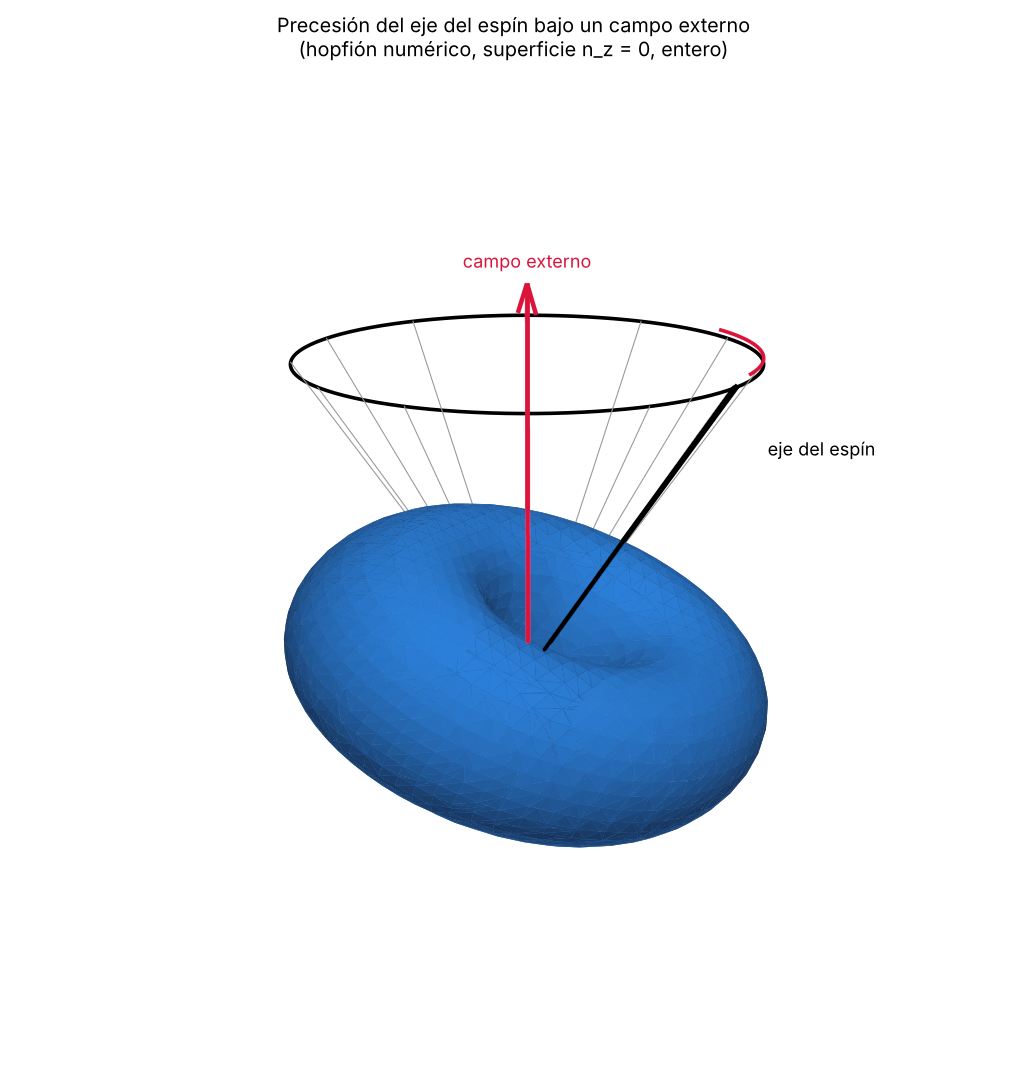
\includegraphics[width=0.5\textwidth]{fig12_precesion.png}
\caption{Precesión del eje del espín bajo un campo externo (punto~3). El hopfión, dibujado entero con su superficie $n_z=0$, tiene el eje inclinado a lo largo de una generatriz del cono, y ese eje gira alrededor de la dirección del campo (flecha roja), a la frecuencia de Larmor. En cambio, avanzar a lo largo de $\eta$ hace girar el toro alrededor de su propio eje, sin precesión. Elaborada con \prog{precesion\_hopfion.py} a partir del hopfión numérico.}
\label{fig:precesion}
\end{figure}

Prueba futura: en el campo de un protón, el nudo debe conservar su tamaño y su carga de Hopf; el orbital es la envolvente, por la que el nudo se mueve (sección~5, puntos 7 y~8). Falta comprobar con un cálculo que el campo de Coulomb a escala atómica no lo deforma de forma apreciable.
% =====================================================================
\section{Conclusiones}

En este trabajo, el espín se interpreta no como un giro en el espacio ordinario, sino como una circulación a velocidad $c$ a lo largo de la dirección compacta $\eta$, con radio $\xi_0$. Esto es posible porque en el hyle las pulsaciones no tienen masa y avanzan a $c$ (postulado~2). En estas condiciones el momento angular sale $m\,\xi_0\,c=\hbar/2$, sin ninguna superficie que supere a $c$, lo que permite superar las contradicciones originales de 1925.

La duplicidad del espín surge de forma natural de la geometría adoptada: el espín es una dirección en las extendidas más el ángulo de la línea que une las nucleaciones periódicas en el plano compacto. Una vuelta completa invierte el signo de la pulsación, y hacen falta dos para volver a la situación inicial.

Esta circulación en $\eta$ es además el origen de la carga eléctrica, fijada por la interfaz A/\Cst, lo que explica su universalidad.

Como en $\xi$ no hay propagación (postulado~1), la ecuación de primer orden se plantea en $4+1$ dimensiones, y $\xi_0$, fijado también por la interfaz A/\Cst, da la masa. Al reducirla se obtiene la ecuación de Dirac con $g=2$ si el marco está anclado a las capas del sustrato, y $g=1$ sin él (Kaluza--Klein ordinario) \st{D, dados los postulados}.

Finalmente, en las extendidas el director forma un hopfión estable, cuyo giro en $\eta$ le da la masa de Kaluza--Klein esperada y un alcance finito, verificado numéricamente.

La ecuación de Dirac describe el espín, pero no ofrece una imagen mecánica de él. Dentro de esta propuesta hemos intentado utilizar un sustrato lo más sencillo posible, pero cada simplificación que hemos probado ha fallado:

Si el sustrato no fuese anisótropo, el perfil radial oscilaría y no existirían las soluciones sin nodos, y sin ellas no hay circulación en $\eta$ ni carga.

Si no añadimos capas que fijen el marco acabamos en un modelo Kaluza--Klein ordinario, que da $g=1$ en vez del $g=2$ experimental.

Si se intenta una descripción sin topología (solitones escalares), estos resultan inestables por el teorema de Derrick: o bien se deshacen, o bien se expanden indefinidamente. La existencia de un director con textura topológica es, por tanto, imprescindible.

Si se intenta un sustrato con respuesta lineal pura (sin umbrales ni nucleaciones) no existe potencial periódico, ni se justifica el uso de la ecuación de Mathieu, ni existe nada en el plano de las compactadas que fije un ángulo.

Por tanto, una imagen mecánica del espín exige al menos un sustrato con capas que fijen el marco, topología que estabilice la partícula y una respuesta no lineal cerca de un punto crítico.

El modelo reúne en una sola imagen propiedades del electrón que en la física actual van por separado. No todas tienen el mismo estatus:

\begin{center}
\small
\begin{tabularx}{\textwidth}{@{}>{\raggedright\arraybackslash}p{0.2\textwidth} Y Y@{}}
\toprule
Propiedad & En el modelo & Estatus \\
\midrule
Espín $\tfrac12$ & Geometría del disco: el marco da una vuelta completa & \st{D} dados los postulados \\
$g=2$ & Marco anclado a las capas & \st{D} dado el postulado~6 \\
Estabilidad & Carga de Hopf $Q=1$ del director & \st{D} y \st{N} \\
Eje del espín & Eje del nudo, heredado por el halo dipolar & \st{N} la forma del halo; \st{H} que sea el eje del espín \\
Ángulo del espín & Línea que une las nucleaciones en el plano compacto & \st{D} los pozos de Mathieu; \st{H} la identificación \\
Tamaño de Compton & Alcance del halo y de la envolvente & \st{H} $k=mc/\hbar$ \\
Radio clásico & Tamaño del nudo, $\ell\approx r_e$ & \st{H} por compatibilidad de escala \\
Apariencia puntual & El nudo se comprime con el choque & \st{D} la ley de escala; \st{H} la dinámica \\
Valor de la carga & Interfaz A/\Cst & \st{D} dado el postulado~5 (universalidad) \\
Campo externo ($1/r^2$ y dipolo) & Flujo medio de la onda estacionaria esférica & \st{H} sin calcular \\
\bottomrule
\end{tabularx}
\end{center}

Sin embargo, todavía quedan varios puntos abiertos \st{A}: durante su desarrollo no hemos conseguido deducir ningún número que no se haya introducido antes como dato (ni la masa, porque $\ell$ y las rigideces $\kappa$ son libres; ni el valor de $\alpha$; ni $g-2$; ni el valor del momento magnético), y ningún observable que la electrodinámica cuántica no prediga ya. Como mucho podemos afirmar que disponemos de una imagen mecánica coherente, que reproduce lo conocido y de la que al menos sabemos dónde podría dejar de hacerlo: la huella de tamaño, del orden de $(\alpha/2)^2$, en el factor de forma (sección~5, punto~5) y un posible acoplamiento de alguna sonda al halo del director.

No podemos olvidar que la lectura geométrica del espín es una hipótesis \st{H}, y $g=2$ depende del postulado~6 (marco anclado), que tiene una motivación mecánica, pero no una demostración. Los problemas abiertos, en particular la anomalía $g-2$ y las condiciones del punto~7 de la sección~5, quedan expuestos para que otros puedan ponerlos a prueba.

El objetivo de este trabajo es ofrecer a las futuras generaciones de físicos una imagen intuitiva del espín que se pueda estudiar, criticar y mejorar. Una idea abierta a la crítica es más útil que una cerrada en falso.

% =====================================================================
\appendix
\renewcommand{\thesection}{\Alph{section}}
\section*{Apéndice A. Reproducibilidad}
\addcontentsline{toc}{section}{Apéndice A. Reproducibilidad}

Todo el código lo ha escrito Claude y lo ha revisado y ejecutado el autor; está disponible en GitHub (\href{https://github.com/ernestoLopezG/leptones-en-el-hyle}{\texttt{ernestoLopezG/leptones-en-el-hyle}}) y en Zenodo, \href{https://doi.org/10.5281/zenodo.23545995}{doi:10.5281/zenodo.23545995}, con licencia MIT y un \texttt{LEEME} que da las órdenes exactas y los valores esperados. Los programas en C++ son un único fichero cada uno, con OpenMP; los análisis están en Python (numpy, scipy, matplotlib, scikit-image). Unidades: $\hbar=c=m=1$ en las carpetas 1 a~4; en la~5, longitudes en $\ell=\sqrt{\kappa_4/\kappa_2}$, $k$ en $1/\ell$ y energías en $\sqrt{\kappa_2\kappa_4}$; en la~6, la ecuación de Mathieu es adimensional.

\begin{center}
\small
\begin{tabularx}{\textwidth}{@{}>{\raggedright\arraybackslash}p{0.29\textwidth} Y Y c@{}}
\toprule
Programa & Qué calcula & Método & Sección \\
\midrule
\prog{hopfion.cpp} & Hopfión de Faddeev--Skyrme, $\int[\partial\vb{n}\cdot\partial\vb{n}+\tfrac12F_{ij}F_{ij}]$ & Flujo de gradiente proyectado sobre la esfera, diferencias centradas, borde $\vb{n}=\hat{\vb{z}}$ & 3 \\
\addlinespace
\prog{hopfion\_eta.cpp} & El mismo, con giro en $\eta$: $+\,k^2\!\int(1-n_z^2)+k^2\!\int|\nabla n_z|^2$ & Ídem & 3 \\
\addlinespace
\prog{hopfion\_quiral.cpp} & Con término quiral en lugar del de cuarto orden & Ídem & 4 \\
\addlinespace
\prog{hopfq.py} & Carga de Hopf $Q=\frac{1}{16\pi^2}\int\vb{A}\cdot\vb{B}$ & $\vb{A}$ desde $\vb{B}$ por FFT (gauge de Coulomb) & 3 \\
\addlinespace
\prog{flujo.py} & Flujo de Mermin--Ho $\vb{v}=\vb{A}$, $\vb{\omega}=\vb{B}$: helicidad y reparto poloidal/toroidal & FFT & 3 \\
\addlinespace
\prog{figura\_hopfion.py} & Figuras de la sección~3 & Isosuperficies (\emph{marching cubes}), líneas de $\vb{\omega}$ integradas & 3 \\
\addlinespace
\prog{medir\_tamano.py} & Radio del anillo y ajuste de la cola, $\ln[r^2(1-n_z)]=\text{cte}-2kr$ & Perfil ecuatorial promediado en ángulo & 3 \\
\addlinespace
\prog{gfactor.py} & $g$ de un director que gira (resultado corregido: $g=1$) & Integrales sobre la solución & 4 \\
\addlinespace
\prog{reposo2}, \prog{umbral}, \prog{evolucion}, \prog{anclada}, \prog{derrick}, \prog{cuartico}, \prog{giro} & Vías escalares descartadas & Ecuación de ondas radial o axisimétrica, diferencias finitas & 4 \\
\addlinespace
\prog{hopfion\_P.cpp} & Giro del director en el tiempo a momento angular fijo, con o sin cuarto orden & Flujo de gradiente con $\omega=S/(2I)$ recalculado en cada paso & 4 \\
\addlinespace
\prog{cola\_angular.py} & Forma angular de la cola: coeficientes de Legendre de $|n_\perp|^2$ en capas esféricas & Mínimos cuadrados por capas & 3 \\
\addlinespace
\prog{reparto\_flujo.py} & Reparto poloidal/toroidal del flujo, en el mapa de Hopf analítico y en las soluciones & FFT & 3 \\
\addlinespace
\prog{figura\_cola\_dipolar.py}, \prog{figura\_espin\_flujo.py} & Figuras ilustrativas: cola dipolar; líneas de flujo de espín $\pm\tfrac12$ e imagen especular & Campos analíticos; enlace por la integral de Gauss & 3 \\
\addlinespace
\prog{precesion\_hopfion.py} & Figura de la precesión del eje bajo un campo externo & Isosuperficie $n_z=0$ de la solución & 5 \\
\addlinespace
\prog{mathieu\_q.py} & Funciones angulares de Mathieu con $q$ negativo y valores característicos de órdenes $0$ y $\tfrac12$ & Método de Hill & 2 \\
\bottomrule
\end{tabularx}
\end{center}

\apartado{Resultados de control} (malla $150^3$, caja~12): $E=544,35$, $E/(32\sqrt2\,\pi^2)=1,219$ (literatura $\approx1,21$), $Q=-0,979$, $E_2/E_4=0,965$; con giro, $E=586,68$ ($k=0,5$) y $675,38$ ($k=1$); $k_{\mathrm{ef}}=1,064$ para $k=1$. El ajuste de la cola se comprobó antes con una cola sintética de $k=1$, que da $1,002$.

\apartado{Comprobaciones que el lector puede repetir.} (1)~Virial: $E_2/E_4\to1$ sin giro, $E_2-E_4+3E_{t2}+E_{t4}\to0$ con giro. (2)~Cota de energía: con $Q=1$ y giro, $E\geq544$; si baja, el nudo se ha deshecho en la malla. (3)~Convergencia en malla: la solución de $100^3$ y la de $150^3$ dan la misma geometría.

\apartado{Límites numéricos.} Con $h=L/(N-1)\gtrsim0,09$ el nudo se deshace incluso sin giro. El esquema es explícito y el término de cuarto orden limita el paso de tiempo en nudos pequeños; los programas con giro reducen el paso solos si la energía sube. Con $k\geq2$ el nudo es más pequeño que lo que resuelven nuestras mallas.

% =====================================================================
\section*{Nota metodológica}
\addcontentsline{toc}{section}{Nota metodológica}

El modelo es fruto de unos veinte años de trabajo del autor. Este trabajo se desarrolló entre junio y octubre de 2026 en colaboración con Claude (Anthropic). El autor aporta la intuición física y la dirección, y tiene la responsabilidad intelectual final; Claude se encargó de la formalización, los programas, la búsqueda bibliográfica y la revisión crítica. Muchos razonamientos se desarrollaron en conversaciones totalmente equivalentes a las que surgirían en cualquier colaboración entre colegas.

Las ciencias naturales son descriptivas, y a menudo tienen que deducir las propiedades de un medio sobre el que no se puede experimentar directamente. Nadie ha estado en el núcleo de la Tierra: su estructura se deduce de cómo viajan las ondas sísmicas, buscando el modelo de interior cuyas soluciones son compatibles con los registros; el interior del Sol se estudia igual, a partir de sus oscilaciones. Este trabajo hace lo mismo con un medio que tampoco se puede observar directamente. Sus afirmaciones tienen la forma de un condicional: «el hyle, sobre el que no podemos experimentar directamente, da soluciones compatibles con lo que observamos si tiene tal propiedad»; por ejemplo, un término de cuarto orden. El punto de partida también es observacional: los electrones existen, tienen naturaleza ondulatoria y se describen como puntuales, sin ninguna estructura en las dimensiones extendidas, lo que es una paradoja física que pide una explicación; buscar las propiedades del medio que permiten esas soluciones es legítimo en un trabajo que no pretende haber resuelto el misterio del espín.

Se ha puesto a cada resultado una etiqueta que permita al lector conocer su estado de desarrollo:

\begin{itemize}[leftmargin=*]
\item \textbf{\st{D} Derivación:} se sigue de los postulados por pasos que el lector puede comprobar.
\item \textbf{\st{H} Hipótesis:} compatible con el modelo y motivada físicamente, pero no derivada.
\item \textbf{\st{N} Numérico:} resultado de un cálculo o una simulación, reproducible con el código público (apéndice~A).
\item \textbf{\st{O} Observación empírica:} un patrón de los datos que el modelo reproduce pero no deriva.
\item \textbf{\st{A} Abierto:} una laguna reconocida, ya sea un problema abierto del modelo o un límite declarado de los cálculos, con lo que haría falta para resolverla.
\end{itemize}

Hemos considerado de utilidad registrar los errores encontrados durante el trabajo y las vías que no funcionaron (sección~4), con su razón.

% =====================================================================
\section*{Referencias}
\addcontentsline{toc}{section}{Referencias}

\begin{list}{}{\setlength{\leftmargin}{1.5em}\setlength{\itemindent}{-1.5em}\setlength{\itemsep}{0.15em}\small}
\item A.~A. Abdo et al., Nature \textbf{462}, 331 (2009).
\item G.~P. Agrawal, \emph{Nonlinear Fiber Optics}, 6.ª ed., Academic Press (2019).
\item J.~C. Alcerro Mena, «Euclidean Equivalent of Minkowski's Space-Time Theory and the Corresponding Model of Elementary Particles (“Cuantex” Model)», Journal of Physics and Astronomy Research \textbf{4}(1), 079--086 (2018).
\item N. Arkani-Hamed, S. Dimopoulos y G. Dvali, Phys. Lett. B \textbf{429}, 263 (1998).
\item J.~E. Avron, R. Seiler y P.~G. Zograf, «Viscosity of quantum Hall fluids», Phys. Rev. Lett. \textbf{75}, 697 (1995).
\item C. Barceló, S. Liberati y M. Visser, «Analogue gravity», Living Rev. Relativ. \textbf{8}, 12 (2005).
\item R.~A. Battye y P.~M. Sutcliffe, Phys. Rev. Lett. \textbf{81}, 4798 (1998).
\item F.~J. Belinfante, «On the spin angular momentum of mesons», Physica \textbf{6}, 887 (1939).
\item J.~S. Bell, «How to teach special relativity», Progress in Scientific Culture \textbf{1} (1976); reimpreso en \emph{Speakable and Unspeakable in Quantum Mechanics}, Cambridge University Press (1987).
\item L. de~Broglie, «La mécanique ondulatoire et la structure atomique de la matière et du rayonnement», J. Phys. Radium \textbf{8}, 225 (1927).
\item G.~H. Derrick, J. Math. Phys. \textbf{5}, 1252 (1964).
\item P.~A.~M. Dirac, «The quantum theory of the electron», Proc. R. Soc. Lond. A \textbf{117}, 610 (1928).
\item M.~J. Duff, J.~T. Liu y J. Rahmfeld, «$g=1$ for Dirichlet 0-branes», Nucl. Phys. B \textbf{524}, 129 (1998), arXiv:hep-th/9801072.
\item L. Faddeev y A.~J. Niemi, «Stable knot-like structures in classical field theory», Nature \textbf{387}, 58 (1997).
\item F. de~Felice, «On the gravitational field acting as an optical medium», Gen. Relativ. Gravit. \textbf{2}, 347 (1971).
\item E. Fermi, J. Pasta y S. Ulam, informe Los Alamos LA-1940 (1955).
\item D. Finkelstein y J. Rubinstein, «Connection between spin, statistics, and kinks», J. Math. Phys. \textbf{9}, 1762 (1968).
\item F.~C. Frank, Proc. Phys. Soc. A \textbf{62}, 131 (1949).
\item P.-G. de~Gennes y J. Prost, \emph{The Physics of Liquid Crystals}, 2.ª ed., Oxford University Press (1993).
\item J.~B. Götte, S.~M. Barnett y M. Padgett, «On the dragging of light by a rotating medium», Proc. R. Soc. A \textbf{463}, 2185 (2007), arXiv:0704.0725.
\item C. Hanhart, J.~A. Pons, D.~R. Phillips y S. Reddy, «The likelihood of GODs' existence: improving the SN 1987a constraint on the size of large compact dimensions», Phys. Lett. B \textbf{509}, 1 (2001), arXiv:astro-ph/0102063.
\item D. Hestenes, «The zitterbewegung interpretation of quantum mechanics», Found. Phys. \textbf{20}, 1213 (1990).
\item A. Hosoya, K. Ishikawa, Y. Ohkuwa y K. Yamagishi, «Gyromagnetic ratio of heavy particles in the Kaluza--Klein theory», Phys. Lett. B \textbf{134}, 44 (1984).
\item R.~V. Jones, «Rotary ‘aether drag’», Proc. R. Soc. Lond. A \textbf{349}, 423 (1976).
\item T. Kaluza, Sitzungsber. Preuss. Akad. Wiss. Berlin, 966 (1921); O. Klein, Z. Phys. \textbf{37}, 895 (1926).
\item W. Thomson (Kelvin), «On vortex atoms», Proc. R. Soc. Edinburgh \textbf{6}, 94 (1867).
\item Y. Koide, «Fermion-boson two-body model of quarks and leptons and Cabibbo mixing», Lett. Nuovo Cimento \textbf{34}, 201 (1982).
\item S. Krusch y J.~M. Speight, «Fermionic quantization of Hopf solitons», Commun. Math. Phys. \textbf{264}, 391 (2006).
\item J.~G. Lee, E.~G. Adelberger, T.~S. Cook, S.~M. Fleischer y B.~R. Heckel, «New test of the gravitational $1/r^2$ law at separations down to 52~$\mu$m», Phys. Rev. Lett. \textbf{124}, 101101 (2020).
\item N.~D. Mermin y T.-L. Ho, Phys. Rev. Lett. \textbf{36}, 594 (1976).
\item H.~K. Moffatt, «The degree of knottedness of tangled vortex lines», J. Fluid Mech. \textbf{35}, 117 (1969).
\item E. Nelson, «Derivation of the Schrödinger equation from Newtonian mechanics», Phys. Rev. \textbf{150}, 1079 (1966).
\item H.~C. Ohanian, «What is spin?», Am. J. Phys. \textbf{54}, 500 (1986).
\item M.~A. Player, «On the dragging of the plane of polarization of light propagating in a rotating medium», Proc. R. Soc. Lond. A \textbf{349}, 441 (1976).
\item A. Prosperetti, J. Acoust. Soc. Am. \textbf{57}, 810 (1975).
\item E. Schrödinger, «Quantisierung als Eigenwertproblem (Vierte Mitteilung)», Ann. Phys. (Leipzig) \textbf{81}, 109 (1926).
\item M. Soler, «Classical, stable, nonlinear spinor field with positive rest energy», Phys. Rev. D \textbf{1}, 2766 (1970).
\item V. Soni et al., «The odd free surface flows of a colloidal chiral fluid», Nature Physics \textbf{15}, 1188 (2019).
\item P. Sutcliffe, «Knots in the Skyrme--Faddeev model», Proc. R. Soc. A \textbf{463}, 3001 (2007), arXiv:0705.1468.
\item G.~E. Uhlenbeck y S. Goudsmit, Naturwissenschaften \textbf{13}, 953 (1925).
\item W.~G. Unruh, Phys. Rev. Lett. \textbf{46}, 1351 (1981).
\item A.~F. Vakulenko y L.~V. Kapitanskii, «Stability of solitons in $S^2$ in the nonlinear $\sigma$-model», Dokl. Akad. Nauk SSSR \textbf{246}, 840 (1979) [Sov. Phys. Dokl. \textbf{24}, 433 (1979)].
\item G.~E. Volovik, \emph{The Universe in a Helium Droplet}, Oxford University Press (2003).
\item G.~E. Volovik y V.~P. Mineev, «Particle-like solitons in superfluid ${}^3$He phases», Zh. Eksp. Teor. Fiz. \textbf{73}, 767 (1977) [Sov. Phys. JETP \textbf{46}, 401 (1977)].
\item E. Witten, «Instability of the Kaluza--Klein vacuum», Nucl. Phys. B \textbf{195}, 481 (1982).
\item E. Witten, «Current algebra, baryons, and quark confinement», Nucl. Phys. B \textbf{223}, 433 (1983).
\item Z. Xi, M. Liu y J. Ulbricht, «New test on contact interactions in the data at $\sqrt{s}=130$--207~GeV by Bhabha scattering process $e^+e^-\to e^+e^-$», arXiv:2411.15686 (2024).
\end{list}

\end{document}
